For our $N$ by $N$ sparse system, we are computing the entire set of $N$ eigenvectors and eigenvalues. The resulting eigenbasis is a dense $N$ by $N$ matrix $V$. The amount of memory required to store $V$ can be excessively large and scales rapidly with respect to the number of elements in the discretization. Therefore some method needed to be employed to reduce the storage requirements and potentially also reduce the amount of work necessary to apply the eigenbasis. In order to compress the data produced by our framework, we utilized Lawrence Livermore's zfp compression library \cite{zfp} to explore different strategies.

Since $V$ is a PETSc matrix that is distributed among all of the available processes, the first compression strategy we explored was to have each process use zfp to compress its local block. This approach doesn't help reduce the amount of work to apply $V$ but it gives us an idea of how much compression is possible using zfp.

The second approach is to compress each eigenvector independently. For any given input function $f$ for the fractional poisson problem, there may be many eigenvectors (if not the majority) that will have scaling coefficients smaller than machine precision. By using this compression strategy, we could only decompress the specific eigenvectors we need for a given $f$ and skip any that will have no effect on the solution. By only keeping the $m$ most recently used eigenvectors in the decompressed state, we could also minimize the amount of time compressing and decompressing eigenvectors.

\subsection{Results}

Using the already computed eigenbasis $V$ for $N = 30^3$, we ran experiments for both compression strategies to determine the time it takes to compress and the amount of data reduction achieved. For the first strategy, we compressed each local block using two evaluators, each with 28 processes. In figures \ref{fig:reduce2} and \ref{fig:compress2}, the results of this experiment can be seen.

\begin{figure}
	\caption{The amount of data reduction achieved by compressing each process's local block.}
	\label{fig:reduce2}
	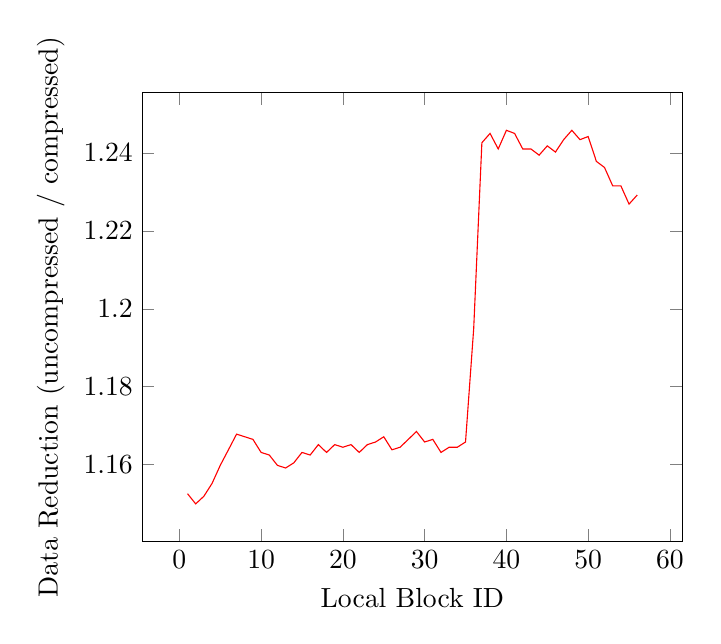
\begin{tikzpicture}
\begin{axis} [xlabel=Local Block ID, ylabel=Data Reduction (uncompressed / compressed)]
\addplot[color=red] coordinates {
(1, 1.1525327262380001)
(2, 1.1499148211240000)
(3, 1.1518771331060000)
(4, 1.1551625784370001)
(5, 1.1597938144330000)
(6, 1.1637931034480000)
(7, 1.1678200692039999)
(8, 1.1671469740630001)
(9, 1.1664746543780000)
(10, 1.1631246410110001)
(11, 1.1624569460390000)
(12, 1.1597938144330000)
(13, 1.1591299370349999)
(14, 1.1604584527220001)
(15, 1.1631246410110001)
(16, 1.1624569460390000)
(17, 1.1651323360179999)
(18, 1.1631246410110001)
(19, 1.1651323360179999)
(20, 1.1644623346750000)
(21, 1.1651323360179999)
(22, 1.1631246410110001)
(23, 1.1651323360179999)
(24, 1.1658031088080001)
(25, 1.1671469740630001)
(26, 1.1637931034480000)
(27, 1.1644623346750000)
(28, 1.1664746543780000)
(29, 1.1684939411430000)
(30, 1.1658031088080001)
(31, 1.1664746543780000)
(32, 1.1631246410110001)
(33, 1.1644623346750000)
(34, 1.1644623346750000)
(35, 1.1658031088080001)
(36, 1.1949305974650000)
(37, 1.2426187419770001)
(38, 1.2450160771700001)
(39, 1.2410256410260001)
(40, 1.2458172458170000)
(41, 1.2450160771700001)
(42, 1.2410256410260001)
(43, 1.2410256410260001)
(44, 1.2394366197180000)
(45, 1.2418216805640001)
(46, 1.2402306213970000)
(47, 1.2434168272320001)
(48, 1.2458172458170000)
(49, 1.2434168272320001)
(50, 1.2442159383030000)
(51, 1.2378516624039999)
(52, 1.2362707535120001)
(53, 1.2315521628499999)
(54, 1.2315521628499999)
(55, 1.2268694550060000)
(56, 1.2292063492059999)
};
\end{axis}
\end{tikzpicture}

\end{figure}

\begin{figure}
	\caption{The amount of time it took to compress each process's local block.}
	\label{fig:compress2}
	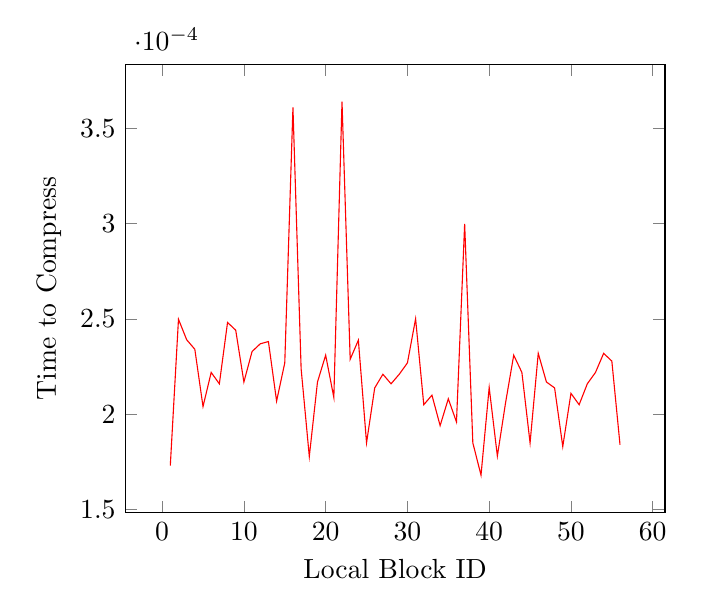
\begin{tikzpicture}
\begin{axis} [xlabel=Local Block ID, ylabel=Time to Compress]
\addplot[color=red] coordinates {
(1, 0.0001730918880000)
(2, 0.0002498626710000)
(3, 0.0002391338350000)
(4, 0.0002341270450000)
(5, 0.0002040863040000)
(6, 0.0002219676970000)
(7, 0.0002160072330000)
(8, 0.0002481937410000)
(9, 0.0002441406250000)
(10, 0.0002169609070000)
(11, 0.0002329349520000)
(12, 0.0002369880680000)
(13, 0.0002381801610000)
(14, 0.0002069473270000)
(15, 0.0002269744870000)
(16, 0.0003609657290000)
(17, 0.0002238750460000)
(18, 0.0001778602600000)
(19, 0.0002169609070000)
(20, 0.0002310276030000)
(21, 0.0002088546750000)
(22, 0.0003640651700000)
(23, 0.0002288818360000)
(24, 0.0002388954160000)
(25, 0.0001850128170000)
(26, 0.0002138614650000)
(27, 0.0002210140230000)
(28, 0.0002160072330000)
(29, 0.0002210140230000)
(30, 0.0002269744870000)
(31, 0.0002501010890000)
(32, 0.0002050399780000)
(33, 0.0002100467680000)
(34, 0.0001940727230000)
(35, 0.0002081394200000)
(36, 0.0001959800720000)
(37, 0.0002999305730000)
(38, 0.0001850128170000)
(39, 0.0001680850980000)
(40, 0.0002140998840000)
(41, 0.0001780986790000)
(42, 0.0002059936520000)
(43, 0.0002310276030000)
(44, 0.0002219676970000)
(45, 0.0001850128170000)
(46, 0.0002319812770000)
(47, 0.0002169609070000)
(48, 0.0002138614650000)
(49, 0.0001831054690000)
(50, 0.0002110004430000)
(51, 0.0002050399780000)
(52, 0.0002160072330000)
(53, 0.0002219676970000)
(54, 0.0002319812770000)
(55, 0.0002279281620000)
(56, 0.0001840591430000)
};
\end{axis}
\end{tikzpicture}

\end{figure}

Then the compression experiment is repeated for strategy 2, where instead of computing the local data blocks, each column of the matrix $V$ is compressed independently. The results of this compression experiment can then be seen in figures \ref{fig:reduce1} and \ref{fig:compress1}.

\begin{figure}
	\caption{The amount of data reduction achieved by compressing each individual eigenvector, sorted in ascending order by eigenvalue.}
	\label{fig:reduce1}
	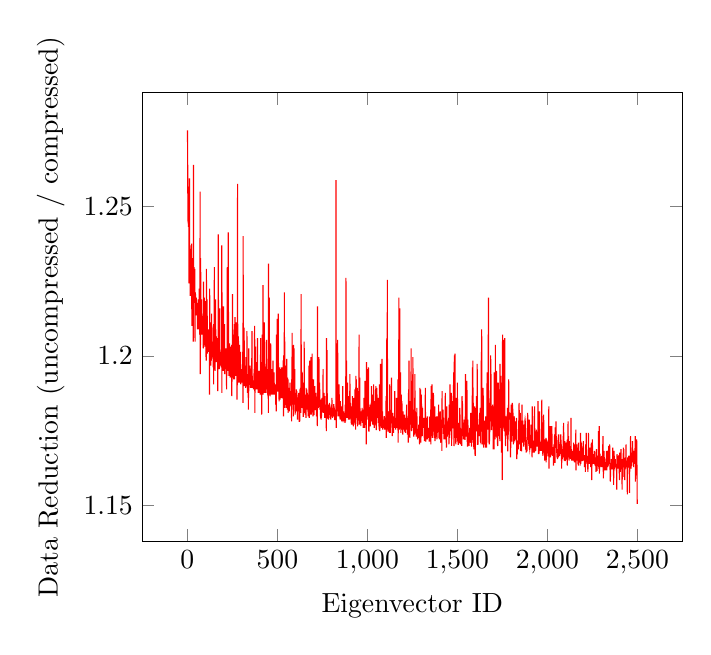
\begin{tikzpicture}
\begin{axis} [xlabel=Eigenvector ID, ylabel=Data Reduction (uncompressed / compressed)]
\addplot[color=red] coordinates {
(1, 1.2755102040820001)
(2, 1.2543903662820000)
(3, 1.2639029322549999)
(4, 1.2444001991039999)
(5, 1.2475049900199999)
(6, 1.2431626056689999)
(7, 1.2525050100199999)
(8, 1.2462612163510001)
(9, 1.2242899118510000)
(10, 1.2512512512509999)
(11, 1.2339585389929999)
(12, 1.2594458438289999)
(13, 1.2345679012349999)
(14, 1.2339585389929999)
(15, 1.2370113805050000)
(16, 1.2201073694489999)
(17, 1.2357884330200000)
(18, 1.2260912211870001)
(19, 1.2339585389929999)
(20, 1.2266928361139999)
(21, 1.2297097884899999)
(22, 1.2260912211870001)
(23, 1.2266928361139999)
(24, 1.2376237623760000)
(25, 1.2100677637949999)
(26, 1.2272950417280000)
(27, 1.2254901960780000)
(28, 1.2195121951220000)
(29, 1.2327416173570001)
(30, 1.2260912211870001)
(31, 1.2291052114059999)
(32, 1.2195121951220000)
(33, 1.2048192771080000)
(34, 1.2639029322549999)
(35, 1.2177301509989999)
(36, 1.2212994626280000)
(37, 1.2297097884899999)
(38, 1.2177301509989999)
(39, 1.2207031250000000)
(40, 1.2201073694489999)
(41, 1.2291052114059999)
(42, 1.2130033964100000)
(43, 1.2048192771080000)
(44, 1.2212994626280000)
(45, 1.2201073694489999)
(46, 1.2207031250000000)
(47, 1.2153621779290000)
(48, 1.2153621779290000)
(49, 1.2189176011700000)
(50, 1.2195121951220000)
(51, 1.2135922330100000)
(52, 1.2177301509989999)
(53, 1.2135922330100000)
(54, 1.2141816415740001)
(55, 1.2165450121650001)
(56, 1.2088974854929999)
(57, 1.2094823415580001)
(58, 1.2130033964100000)
(59, 1.2159533073930000)
(60, 1.2189176011700000)
(61, 1.2100677637949999)
(62, 1.2135922330100000)
(63, 1.2135922330100000)
(64, 1.2147716229350001)
(65, 1.2088974854929999)
(66, 1.2224938875310001)
(67, 1.2153621779290000)
(68, 1.2106537530270001)
(69, 1.2071463061320000)
(70, 1.2135922330100000)
(71, 1.2550200803210001)
(72, 1.1938872970390000)
(73, 1.2059816690790000)
(74, 1.2327416173570001)
(75, 1.2088974854929999)
(76, 1.2124151309410001)
(77, 1.2130033964100000)
(78, 1.2071463061320000)
(79, 1.2189176011700000)
(80, 1.2094823415580001)
(81, 1.2141816415740001)
(82, 1.2083131947800001)
(83, 1.2071463061320000)
(84, 1.2077294685990001)
(85, 1.2088974854929999)
(86, 1.2130033964100000)
(87, 1.2088974854929999)
(88, 1.2030798845040001)
(89, 1.2025012025010000)
(90, 1.2248897599220001)
(91, 1.2030798845040001)
(92, 1.2042389210019999)
(93, 1.2159533073930000)
(94, 1.2195121951220000)
(95, 1.2059816690790000)
(96, 1.2036591237359999)
(97, 1.2083131947800001)
(98, 1.2065637065640000)
(99, 1.2112403100780000)
(100, 1.2030798845040001)
(101, 1.2183235867450000)
(102, 1.2042389210019999)
(103, 1.2130033964100000)
(104, 1.1990407673860000)
(105, 1.1984659635670001)
(106, 1.2291052114059999)
(107, 1.2013455069679999)
(108, 1.2013455069679999)
(109, 1.2059816690790000)
(110, 1.2189176011700000)
(111, 1.2007684918349999)
(112, 1.2088974854929999)
(113, 1.2042389210019999)
(114, 1.2065637065640000)
(115, 1.2065637065640000)
(116, 1.2019230769230000)
(117, 1.2019230769230000)
(118, 1.2088974854929999)
(119, 1.2013455069679999)
(120, 1.2054001928639999)
(121, 1.2042389210019999)
(122, 1.2030798845040001)
(123, 1.1870845204180001)
(124, 1.2224938875310001)
(125, 1.2106537530270001)
(126, 1.2001920307250000)
(127, 1.2030798845040001)
(128, 1.1978917105889999)
(129, 1.2065637065640000)
(130, 1.2013455069679999)
(131, 1.1967448539970000)
(132, 1.2112403100780000)
(133, 1.1984659635670001)
(134, 1.1996161228410001)
(135, 1.2141816415740001)
(136, 1.2007684918349999)
(137, 1.2048192771080000)
(138, 1.2036591237359999)
(139, 1.2001920307250000)
(140, 1.2013455069679999)
(141, 1.2030798845040001)
(142, 1.1990407673860000)
(143, 1.2042389210019999)
(144, 1.1961722488040001)
(145, 1.2094823415580001)
(146, 1.1904761904760000)
(147, 1.2106537530270001)
(148, 1.1996161228410001)
(149, 1.2100677637949999)
(150, 1.2297097884899999)
(151, 1.2001920307250000)
(152, 1.2048192771080000)
(153, 1.2025012025010000)
(154, 1.1950286806879999)
(155, 1.2059816690790000)
(156, 1.1996161228410001)
(157, 1.2189176011700000)
(158, 1.1996161228410001)
(159, 1.2030798845040001)
(160, 1.1978917105889999)
(161, 1.2065637065640000)
(162, 1.1996161228410001)
(163, 1.1978917105889999)
(164, 1.2059816690790000)
(165, 1.1978917105889999)
(166, 1.2025012025010000)
(167, 1.2042389210019999)
(168, 1.2001920307250000)
(169, 1.1882129277569999)
(170, 1.1973180076629999)
(171, 1.1978917105889999)
(172, 1.2406947890819999)
(173, 1.2130033964100000)
(174, 1.1978917105889999)
(175, 1.2094823415580001)
(176, 1.1990407673860000)
(177, 1.1956001912959999)
(178, 1.2030798845040001)
(179, 1.1967448539970000)
(180, 1.2159533073930000)
(181, 1.1973180076629999)
(182, 1.1990407673860000)
(183, 1.1967448539970000)
(184, 1.2013455069679999)
(185, 1.1978917105889999)
(186, 1.1984659635670001)
(187, 1.1990407673860000)
(188, 1.1961722488040001)
(189, 1.1967448539970000)
(190, 1.2001920307250000)
(191, 1.2370113805050000)
(192, 1.1876484560570000)
(193, 1.2212994626280000)
(194, 1.1956001912959999)
(195, 1.1967448539970000)
(196, 1.1996161228410001)
(197, 1.2019230769230000)
(198, 1.1967448539970000)
(199, 1.1950286806879999)
(200, 1.2077294685990001)
(201, 1.2165450121650001)
(202, 1.1961722488040001)
(203, 1.1996161228410001)
(204, 1.1961722488040001)
(205, 1.1978917105889999)
(206, 1.1950286806879999)
(207, 1.2106537530270001)
(208, 1.1938872970390000)
(209, 1.1973180076629999)
(210, 1.1978917105889999)
(211, 1.2019230769230000)
(212, 1.1961722488040001)
(213, 1.2007684918349999)
(214, 1.1956001912959999)
(215, 1.2025012025010000)
(216, 1.1961722488040001)
(217, 1.1961722488040001)
(218, 1.1887779362819999)
(219, 1.1961722488040001)
(220, 1.1956001912959999)
(221, 1.1956001912959999)
(222, 1.2297097884899999)
(223, 1.1950286806879999)
(224, 1.1961722488040001)
(225, 1.1984659635670001)
(226, 1.1961722488040001)
(227, 1.2413108242299999)
(228, 1.2248897599220001)
(229, 1.1950286806879999)
(230, 1.1978917105889999)
(231, 1.1933174224340000)
(232, 1.1961722488040001)
(233, 1.1996161228410001)
(234, 1.2042389210019999)
(235, 1.1933174224340000)
(236, 1.1956001912959999)
(237, 1.2025012025010000)
(238, 1.1927480916030000)
(239, 1.1956001912959999)
(240, 1.1956001912959999)
(241, 1.1944577161970000)
(242, 1.2030798845040001)
(243, 1.1950286806879999)
(244, 1.1950286806879999)
(245, 1.1933174224340000)
(246, 1.2036591237359999)
(247, 1.1865211200760000)
(248, 1.1927480916030000)
(249, 1.1990407673860000)
(250, 1.1933174224340000)
(251, 1.2207031250000000)
(252, 1.1933174224340000)
(253, 1.1933174224340000)
(254, 1.1961722488040001)
(255, 1.1927480916030000)
(256, 1.1984659635670001)
(257, 1.1921793037670001)
(258, 1.2071463061320000)
(259, 1.1984659635670001)
(260, 1.1956001912959999)
(261, 1.2106537530270001)
(262, 1.1921793037670001)
(263, 1.1950286806879999)
(264, 1.1961722488040001)
(265, 1.2130033964100000)
(266, 1.1933174224340000)
(267, 1.1938872970390000)
(268, 1.2054001928639999)
(269, 1.1933174224340000)
(270, 1.1967448539970000)
(271, 1.1938872970390000)
(272, 1.2112403100780000)
(273, 1.1973180076629999)
(274, 1.1938872970390000)
(275, 1.1944577161970000)
(276, 1.1853959222379999)
(277, 1.1904761904760000)
(278, 1.1938872970390000)
(279, 1.2575452716300000)
(280, 1.1927480916030000)
(281, 1.1996161228410001)
(282, 1.1921793037670001)
(283, 1.2065637065640000)
(284, 1.2048192771080000)
(285, 1.1910433539780001)
(286, 1.1950286806879999)
(287, 1.1933174224340000)
(288, 1.1916110581510000)
(289, 1.1933174224340000)
(290, 1.2036591237359999)
(291, 1.1910433539780001)
(292, 1.1938872970390000)
(293, 1.2001920307250000)
(294, 1.1996161228410001)
(295, 1.1916110581510000)
(296, 1.2013455069679999)
(297, 1.1904761904760000)
(298, 1.1938872970390000)
(299, 1.1933174224340000)
(300, 1.1950286806879999)
(301, 1.1938872970390000)
(302, 1.1916110581510000)
(303, 1.1956001912959999)
(304, 1.1927480916030000)
(305, 1.1910433539780001)
(306, 1.1938872970390000)
(307, 1.1933174224340000)
(308, 1.2013455069679999)
(309, 1.1842728564659999)
(310, 1.2400793650790001)
(311, 1.1927480916030000)
(312, 1.2077294685990001)
(313, 1.1899095668730000)
(314, 1.1904761904760000)
(315, 1.2094823415580001)
(316, 1.2042389210019999)
(317, 1.1899095668730000)
(318, 1.1927480916030000)
(319, 1.1927480916030000)
(320, 1.1927480916030000)
(321, 1.1899095668730000)
(322, 1.1944577161970000)
(323, 1.1967448539970000)
(324, 1.1893434823980000)
(325, 1.1904761904760000)
(326, 1.1996161228410001)
(327, 1.1916110581510000)
(328, 1.1910433539780001)
(329, 1.1899095668730000)
(330, 1.1950286806879999)
(331, 1.2083131947800001)
(332, 1.1916110581510000)
(333, 1.1938872970390000)
(334, 1.1876484560570000)
(335, 1.1899095668730000)
(336, 1.1921793037670001)
(337, 1.1916110581510000)
(338, 1.1933174224340000)
(339, 1.1820330969270001)
(340, 1.1910433539780001)
(341, 1.2025012025010000)
(342, 1.1882129277569999)
(343, 1.1938872970390000)
(344, 1.1933174224340000)
(345, 1.1910433539780001)
(346, 1.1904761904760000)
(347, 1.1904761904760000)
(348, 1.1933174224340000)
(349, 1.1967448539970000)
(350, 1.1904761904760000)
(351, 1.1944577161970000)
(352, 1.1893434823980000)
(353, 1.1899095668730000)
(354, 1.1904761904760000)
(355, 1.1893434823980000)
(356, 1.1927480916030000)
(357, 1.1904761904760000)
(358, 1.1984659635670001)
(359, 1.2083131947800001)
(360, 1.1899095668730000)
(361, 1.1933174224340000)
(362, 1.1893434823980000)
(363, 1.1904761904760000)
(364, 1.1916110581510000)
(365, 1.1916110581510000)
(366, 1.1904761904760000)
(367, 1.1887779362819999)
(368, 1.1916110581510000)
(369, 1.1887779362819999)
(370, 1.1921793037670001)
(371, 1.1956001912959999)
(372, 1.1887779362819999)
(373, 1.2065637065640000)
(374, 1.2100677637949999)
(375, 1.1809163911200000)
(376, 1.1933174224340000)
(377, 1.1916110581510000)
(378, 1.1893434823980000)
(379, 1.2030798845040001)
(380, 1.1893434823980000)
(381, 1.1910433539780001)
(382, 1.1887779362819999)
(383, 1.1978917105889999)
(384, 1.1893434823980000)
(385, 1.1904761904760000)
(386, 1.1927480916030000)
(387, 1.1927480916030000)
(388, 1.1978917105889999)
(389, 1.1887779362819999)
(390, 1.2059816690790000)
(391, 1.1899095668730000)
(392, 1.1933174224340000)
(393, 1.1893434823980000)
(394, 1.1876484560570000)
(395, 1.1899095668730000)
(396, 1.1938872970390000)
(397, 1.1876484560570000)
(398, 1.1950286806879999)
(399, 1.1910433539780001)
(400, 1.1887779362819999)
(401, 1.1876484560570000)
(402, 1.1927480916030000)
(403, 1.1876484560570000)
(404, 1.1916110581510000)
(405, 1.1870845204180001)
(406, 1.1882129277569999)
(407, 1.2059816690790000)
(408, 1.1876484560570000)
(409, 1.1978917105889999)
(410, 1.1899095668730000)
(411, 1.1882129277569999)
(412, 1.1887779362819999)
(413, 1.1803588290839999)
(414, 1.1876484560570000)
(415, 1.1887779362819999)
(416, 1.2071463061320000)
(417, 1.1887779362819999)
(418, 1.1893434823980000)
(419, 1.1910433539780001)
(420, 1.2236906510029999)
(421, 1.1870845204180001)
(422, 1.1927480916030000)
(423, 1.1899095668730000)
(424, 1.1882129277569999)
(425, 1.1893434823980000)
(426, 1.1876484560570000)
(427, 1.1899095668730000)
(428, 1.2112403100780000)
(429, 1.1904761904760000)
(430, 1.1938872970390000)
(431, 1.1973180076629999)
(432, 1.1876484560570000)
(433, 1.1938872970390000)
(434, 1.1876484560570000)
(435, 1.1882129277569999)
(436, 1.1882129277569999)
(437, 1.1876484560570000)
(438, 1.1887779362819999)
(439, 1.1899095668730000)
(440, 1.2054001928639999)
(441, 1.1916110581510000)
(442, 1.1893434823980000)
(443, 1.1904761904760000)
(444, 1.1944577161970000)
(445, 1.1927480916030000)
(446, 1.1870845204180001)
(447, 1.1956001912959999)
(448, 1.1865211200760000)
(449, 1.1990407673860000)
(450, 1.1809163911200000)
(451, 1.2309207287049999)
(452, 1.1899095668730000)
(453, 1.1870845204180001)
(454, 1.1887779362819999)
(455, 1.2195121951220000)
(456, 1.1899095668730000)
(457, 1.1870845204180001)
(458, 1.1904761904760000)
(459, 1.1865211200760000)
(460, 1.1870845204180001)
(461, 1.1904761904760000)
(462, 1.1882129277569999)
(463, 1.2042389210019999)
(464, 1.1893434823980000)
(465, 1.1899095668730000)
(466, 1.1870845204180001)
(467, 1.1921793037670001)
(468, 1.1893434823980000)
(469, 1.1910433539780001)
(470, 1.1956001912959999)
(471, 1.1893434823980000)
(472, 1.1870845204180001)
(473, 1.1927480916030000)
(474, 1.1882129277569999)
(475, 1.1893434823980000)
(476, 1.1984659635670001)
(477, 1.1876484560570000)
(478, 1.1876484560570000)
(479, 1.1870845204180001)
(480, 1.1944577161970000)
(481, 1.1882129277569999)
(482, 1.1944577161970000)
(483, 1.1870845204180001)
(484, 1.1882129277569999)
(485, 1.1876484560570000)
(486, 1.1876484560570000)
(487, 1.1876484560570000)
(488, 1.1904761904760000)
(489, 1.1893434823980000)
(490, 1.1870845204180001)
(491, 1.1837121212120001)
(492, 1.1870845204180001)
(493, 1.1876484560570000)
(494, 1.1814744801510000)
(495, 1.2071463061320000)
(496, 1.2025012025010000)
(497, 1.1882129277569999)
(498, 1.1904761904760000)
(499, 1.2124151309410001)
(500, 1.1899095668730000)
(501, 1.1882129277569999)
(502, 1.1882129277569999)
(503, 1.1944577161970000)
(504, 1.1916110581510000)
(505, 1.2141816415740001)
(506, 1.1984659635670001)
(507, 1.1887779362819999)
(508, 1.1893434823980000)
(509, 1.1859582542689999)
(510, 1.1848341232230000)
(511, 1.1870845204180001)
(512, 1.1961722488040001)
(513, 1.1882129277569999)
(514, 1.1893434823980000)
(515, 1.1853959222379999)
(516, 1.1882129277569999)
(517, 1.1956001912959999)
(518, 1.1876484560570000)
(519, 1.1927480916030000)
(520, 1.1870845204180001)
(521, 1.1870845204180001)
(522, 1.1859582542689999)
(523, 1.1961722488040001)
(524, 1.1870845204180001)
(525, 1.1859582542689999)
(526, 1.1870845204180001)
(527, 1.1859582542689999)
(528, 1.1859582542689999)
(529, 1.1870845204180001)
(530, 1.1921793037670001)
(531, 1.1916110581510000)
(532, 1.1984659635670001)
(533, 1.1978917105889999)
(534, 1.1798017932989999)
(535, 1.2001920307250000)
(536, 1.1825922421949999)
(537, 1.1870845204180001)
(538, 1.1865211200760000)
(539, 1.2212994626280000)
(540, 1.1848341232230000)
(541, 1.2048192771080000)
(542, 1.1825922421949999)
(543, 1.1882129277569999)
(544, 1.1870845204180001)
(545, 1.1859582542689999)
(546, 1.1848341232230000)
(547, 1.1967448539970000)
(548, 1.1899095668730000)
(549, 1.1904761904760000)
(550, 1.1870845204180001)
(551, 1.1825922421949999)
(552, 1.1990407673860000)
(553, 1.1853959222379999)
(554, 1.1853959222379999)
(555, 1.1842728564659999)
(556, 1.1820330969270001)
(557, 1.1927480916030000)
(558, 1.1876484560570000)
(559, 1.1921793037670001)
(560, 1.1809163911200000)
(561, 1.1882129277569999)
(562, 1.1842728564659999)
(563, 1.1853959222379999)
(564, 1.1848341232230000)
(565, 1.1882129277569999)
(566, 1.1814744801510000)
(567, 1.1893434823980000)
(568, 1.1870845204180001)
(569, 1.1876484560570000)
(570, 1.1910433539780001)
(571, 1.1887779362819999)
(572, 1.1859582542689999)
(573, 1.1848341232230000)
(574, 1.1842728564659999)
(575, 1.1831519167060001)
(576, 1.1848341232230000)
(577, 1.1848341232230000)
(578, 1.1882129277569999)
(579, 1.1781338360039999)
(580, 1.1921793037670001)
(581, 1.1837121212120001)
(582, 1.2077294685990001)
(583, 1.1848341232230000)
(584, 1.1870845204180001)
(585, 1.1837121212120001)
(586, 1.1848341232230000)
(587, 1.1848341232230000)
(588, 1.1853959222379999)
(589, 1.1798017932989999)
(590, 1.2036591237359999)
(591, 1.1842728564659999)
(592, 1.1848341232230000)
(593, 1.2025012025010000)
(594, 1.1842728564659999)
(595, 1.1848341232230000)
(596, 1.1837121212120001)
(597, 1.1956001912959999)
(598, 1.1820330969270001)
(599, 1.1803588290839999)
(600, 1.1853959222379999)
(601, 1.1859582542689999)
(602, 1.1870845204180001)
(603, 1.1876484560570000)
(604, 1.1865211200760000)
(605, 1.1859582542689999)
(606, 1.1887779362819999)
(607, 1.1814744801510000)
(608, 1.1882129277569999)
(609, 1.1848341232230000)
(610, 1.1842728564659999)
(611, 1.1814744801510000)
(612, 1.1786892975009999)
(613, 1.1820330969270001)
(614, 1.1859582542689999)
(615, 1.1859582542689999)
(616, 1.1814744801510000)
(617, 1.1848341232230000)
(618, 1.1876484560570000)
(619, 1.1865211200760000)
(620, 1.1865211200760000)
(621, 1.1781338360039999)
(622, 1.1781338360039999)
(623, 1.1848341232230000)
(624, 1.1853959222379999)
(625, 1.1781338360039999)
(626, 1.1887779362819999)
(627, 1.1837121212120001)
(628, 1.1893434823980000)
(629, 1.1842728564659999)
(630, 1.1809163911200000)
(631, 1.1865211200760000)
(632, 1.2207031250000000)
(633, 1.1831519167060001)
(634, 1.1950286806879999)
(635, 1.1848341232230000)
(636, 1.1853959222379999)
(637, 1.1825922421949999)
(638, 1.1944577161970000)
(639, 1.1865211200760000)
(640, 1.1876484560570000)
(641, 1.1831519167060001)
(642, 1.1910433539780001)
(643, 1.1798017932989999)
(644, 1.1798017932989999)
(645, 1.1876484560570000)
(646, 1.1820330969270001)
(647, 1.1876484560570000)
(648, 1.1842728564659999)
(649, 1.2048192771080000)
(650, 1.1859582542689999)
(651, 1.1853959222379999)
(652, 1.1809163911200000)
(653, 1.1859582542689999)
(654, 1.1837121212120001)
(655, 1.1803588290839999)
(656, 1.1870845204180001)
(657, 1.1842728564659999)
(658, 1.1848341232230000)
(659, 1.1792452830189999)
(660, 1.1893434823980000)
(661, 1.1842728564659999)
(662, 1.1837121212120001)
(663, 1.1887779362819999)
(664, 1.1820330969270001)
(665, 1.1831519167060001)
(666, 1.1831519167060001)
(667, 1.1876484560570000)
(668, 1.1842728564659999)
(669, 1.1853959222379999)
(670, 1.1831519167060001)
(671, 1.1798017932989999)
(672, 1.1809163911200000)
(673, 1.1853959222379999)
(674, 1.1859582542689999)
(675, 1.1837121212120001)
(676, 1.1967448539970000)
(677, 1.1792452830189999)
(678, 1.1814744801510000)
(679, 1.1848341232230000)
(680, 1.1984659635670001)
(681, 1.1837121212120001)
(682, 1.1842728564659999)
(683, 1.1859582542689999)
(684, 1.1803588290839999)
(685, 1.1842728564659999)
(686, 1.1996161228410001)
(687, 1.1820330969270001)
(688, 1.1803588290839999)
(689, 1.1825922421949999)
(690, 1.1837121212120001)
(691, 1.1837121212120001)
(692, 1.1842728564659999)
(693, 1.2007684918349999)
(694, 1.1853959222379999)
(695, 1.1853959222379999)
(696, 1.1837121212120001)
(697, 1.1809163911200000)
(698, 1.1798017932989999)
(699, 1.1848341232230000)
(700, 1.1842728564659999)
(701, 1.1921793037670001)
(702, 1.1853959222379999)
(703, 1.1803588290839999)
(704, 1.1803588290839999)
(705, 1.1882129277569999)
(706, 1.1876484560570000)
(707, 1.1859582542689999)
(708, 1.1899095668730000)
(709, 1.1820330969270001)
(710, 1.1820330969270001)
(711, 1.1870845204180001)
(712, 1.1825922421949999)
(713, 1.1842728564659999)
(714, 1.1876484560570000)
(715, 1.1842728564659999)
(716, 1.1842728564659999)
(717, 1.1798017932989999)
(718, 1.1842728564659999)
(719, 1.1859582542689999)
(720, 1.1798017932989999)
(721, 1.1814744801510000)
(722, 1.1764705882349999)
(723, 1.2165450121650001)
(724, 1.1820330969270001)
(725, 1.1956001912959999)
(726, 1.1916110581510000)
(727, 1.1825922421949999)
(728, 1.1882129277569999)
(729, 1.1831519167060001)
(730, 1.1831519167060001)
(731, 1.1996161228410001)
(732, 1.1853959222379999)
(733, 1.1882129277569999)
(734, 1.1910433539780001)
(735, 1.1842728564659999)
(736, 1.1887779362819999)
(737, 1.1820330969270001)
(738, 1.1853959222379999)
(739, 1.1798017932989999)
(740, 1.1803588290839999)
(741, 1.1792452830189999)
(742, 1.1798017932989999)
(743, 1.1786892975009999)
(744, 1.1798017932989999)
(745, 1.1798017932989999)
(746, 1.1803588290839999)
(747, 1.1859582542689999)
(748, 1.1814744801510000)
(749, 1.1809163911200000)
(750, 1.1848341232230000)
(751, 1.1831519167060001)
(752, 1.1831519167060001)
(753, 1.1814744801510000)
(754, 1.1956001912959999)
(755, 1.1825922421949999)
(756, 1.1837121212120001)
(757, 1.1831519167060001)
(758, 1.1809163911200000)
(759, 1.1814744801510000)
(760, 1.1876484560570000)
(761, 1.1825922421949999)
(762, 1.1865211200760000)
(763, 1.1792452830189999)
(764, 1.1803588290839999)
(765, 1.1820330969270001)
(766, 1.1798017932989999)
(767, 1.1798017932989999)
(768, 1.1837121212120001)
(769, 1.1814744801510000)
(770, 1.1792452830189999)
(771, 1.1865211200760000)
(772, 1.1748120300750000)
(773, 1.2059816690790000)
(774, 1.1825922421949999)
(775, 1.1825922421949999)
(776, 1.2019230769230000)
(777, 1.1853959222379999)
(778, 1.1820330969270001)
(779, 1.1792452830189999)
(780, 1.1792452830189999)
(781, 1.1831519167060001)
(782, 1.1831519167060001)
(783, 1.1792452830189999)
(784, 1.1786892975009999)
(785, 1.1837121212120001)
(786, 1.1809163911200000)
(787, 1.1814744801510000)
(788, 1.1831519167060001)
(789, 1.1842728564659999)
(790, 1.1837121212120001)
(791, 1.1814744801510000)
(792, 1.1831519167060001)
(793, 1.1792452830189999)
(794, 1.1803588290839999)
(795, 1.1809163911200000)
(796, 1.1803588290839999)
(797, 1.1786892975009999)
(798, 1.1798017932989999)
(799, 1.1803588290839999)
(800, 1.1837121212120001)
(801, 1.1798017932989999)
(802, 1.1809163911200000)
(803, 1.1859582542689999)
(804, 1.1831519167060001)
(805, 1.1798017932989999)
(806, 1.1814744801510000)
(807, 1.1792452830189999)
(808, 1.1803588290839999)
(809, 1.1809163911200000)
(810, 1.1820330969270001)
(811, 1.1825922421949999)
(812, 1.1809163911200000)
(813, 1.1837121212120001)
(814, 1.1837121212120001)
(815, 1.1820330969270001)
(816, 1.1798017932989999)
(817, 1.1825922421949999)
(818, 1.1786892975009999)
(819, 1.1786892975009999)
(820, 1.1803588290839999)
(821, 1.1798017932989999)
(822, 1.1809163911200000)
(823, 1.1792452830189999)
(824, 1.1792452830189999)
(825, 1.1786892975009999)
(826, 1.2588116817720001)
(827, 1.1759172154280000)
(828, 1.1825922421949999)
(829, 1.2042389210019999)
(830, 1.1814744801510000)
(831, 1.1882129277569999)
(832, 1.1820330969270001)
(833, 1.1859582542689999)
(834, 1.1831519167060001)
(835, 1.2054001928639999)
(836, 1.1837121212120001)
(837, 1.1798017932989999)
(838, 1.1809163911200000)
(839, 1.1899095668730000)
(840, 1.1798017932989999)
(841, 1.1837121212120001)
(842, 1.1803588290839999)
(843, 1.1904761904760000)
(844, 1.1842728564659999)
(845, 1.1798017932989999)
(846, 1.1825922421949999)
(847, 1.1820330969270001)
(848, 1.1792452830189999)
(849, 1.1786892975009999)
(850, 1.1848341232230000)
(851, 1.1825922421949999)
(852, 1.1798017932989999)
(853, 1.1786892975009999)
(854, 1.1792452830189999)
(855, 1.1803588290839999)
(856, 1.1809163911200000)
(857, 1.1781338360039999)
(858, 1.1798017932989999)
(859, 1.1831519167060001)
(860, 1.1781338360039999)
(861, 1.1792452830189999)
(862, 1.1809163911200000)
(863, 1.1899095668730000)
(864, 1.1798017932989999)
(865, 1.1792452830189999)
(866, 1.1798017932989999)
(867, 1.1803588290839999)
(868, 1.1814744801510000)
(869, 1.1792452830189999)
(870, 1.1803588290839999)
(871, 1.1781338360039999)
(872, 1.1792452830189999)
(873, 1.1809163911200000)
(874, 1.1792452830189999)
(875, 1.1792452830189999)
(876, 1.1775788977860000)
(877, 1.1837121212120001)
(878, 1.1792452830189999)
(879, 1.1781338360039999)
(880, 1.1831519167060001)
(881, 1.2260912211870001)
(882, 1.1853959222379999)
(883, 1.1814744801510000)
(884, 1.1984659635670001)
(885, 1.1831519167060001)
(886, 1.1792452830189999)
(887, 1.1848341232230000)
(888, 1.1792452830189999)
(889, 1.1803588290839999)
(890, 1.1910433539780001)
(891, 1.1842728564659999)
(892, 1.1792452830189999)
(893, 1.1798017932989999)
(894, 1.1798017932989999)
(895, 1.1786892975009999)
(896, 1.1798017932989999)
(897, 1.1865211200760000)
(898, 1.1798017932989999)
(899, 1.1809163911200000)
(900, 1.1792452830189999)
(901, 1.1786892975009999)
(902, 1.1837121212120001)
(903, 1.1938872970390000)
(904, 1.1809163911200000)
(905, 1.1798017932989999)
(906, 1.1842728564659999)
(907, 1.1792452830189999)
(908, 1.1792452830189999)
(909, 1.1803588290839999)
(910, 1.1775788977860000)
(911, 1.1831519167060001)
(912, 1.1770244821089999)
(913, 1.1792452830189999)
(914, 1.1770244821089999)
(915, 1.1781338360039999)
(916, 1.1792452830189999)
(917, 1.1865211200760000)
(918, 1.1814744801510000)
(919, 1.1786892975009999)
(920, 1.1786892975009999)
(921, 1.1781338360039999)
(922, 1.1764705882349999)
(923, 1.1781338360039999)
(924, 1.1770244821089999)
(925, 1.1859582542689999)
(926, 1.1853959222379999)
(927, 1.1781338360039999)
(928, 1.1792452830189999)
(929, 1.1831519167060001)
(930, 1.1820330969270001)
(931, 1.1887779362819999)
(932, 1.1803588290839999)
(933, 1.1770244821089999)
(934, 1.1786892975009999)
(935, 1.1753643629530000)
(936, 1.1933174224340000)
(937, 1.1809163911200000)
(938, 1.1910433539780001)
(939, 1.1921793037670001)
(940, 1.1792452830189999)
(941, 1.1825922421949999)
(942, 1.1809163911200000)
(943, 1.1792452830189999)
(944, 1.1893434823980000)
(945, 1.1781338360039999)
(946, 1.1764705882349999)
(947, 1.1781338360039999)
(948, 1.1882129277569999)
(949, 1.1809163911200000)
(950, 1.1814744801510000)
(951, 1.1882129277569999)
(952, 1.1809163911200000)
(953, 1.1825922421949999)
(954, 1.2071463061320000)
(955, 1.1786892975009999)
(956, 1.1770244821089999)
(957, 1.1792452830189999)
(958, 1.1927480916030000)
(959, 1.1798017932989999)
(960, 1.1814744801510000)
(961, 1.1798017932989999)
(962, 1.1775788977860000)
(963, 1.1814744801510000)
(964, 1.1764705882349999)
(965, 1.1814744801510000)
(966, 1.1792452830189999)
(967, 1.1809163911200000)
(968, 1.1798017932989999)
(969, 1.1814744801510000)
(970, 1.1809163911200000)
(971, 1.1825922421949999)
(972, 1.1775788977860000)
(973, 1.1814744801510000)
(974, 1.1820330969270001)
(975, 1.1803588290839999)
(976, 1.1792452830189999)
(977, 1.1759172154280000)
(978, 1.1792452830189999)
(979, 1.1798017932989999)
(980, 1.1786892975009999)
(981, 1.1859582542689999)
(982, 1.1837121212120001)
(983, 1.1814744801510000)
(984, 1.1781338360039999)
(985, 1.1759172154280000)
(986, 1.1814744801510000)
(987, 1.1916110581510000)
(988, 1.1775788977860000)
(989, 1.1770244821089999)
(990, 1.1786892975009999)
(991, 1.1770244821089999)
(992, 1.1809163911200000)
(993, 1.1786892975009999)
(994, 1.1704119850190000)
(995, 1.1978917105889999)
(996, 1.1950286806879999)
(997, 1.1792452830189999)
(998, 1.1786892975009999)
(999, 1.1899095668730000)
(1000, 1.1798017932989999)
(1001, 1.1803588290839999)
(1002, 1.1803588290839999)
(1003, 1.1956001912959999)
(1004, 1.1809163911200000)
(1005, 1.1876484560570000)
(1006, 1.1961722488040001)
(1007, 1.1798017932989999)
(1008, 1.1748120300750000)
(1009, 1.1748120300750000)
(1010, 1.1837121212120001)
(1011, 1.1786892975009999)
(1012, 1.1781338360039999)
(1013, 1.1781338360039999)
(1014, 1.1814744801510000)
(1015, 1.1775788977860000)
(1016, 1.1770244821089999)
(1017, 1.1764705882349999)
(1018, 1.1837121212120001)
(1019, 1.1809163911200000)
(1020, 1.1792452830189999)
(1021, 1.1842728564659999)
(1022, 1.1786892975009999)
(1023, 1.1899095668730000)
(1024, 1.1786892975009999)
(1025, 1.1781338360039999)
(1026, 1.1803588290839999)
(1027, 1.1848341232230000)
(1028, 1.1825922421949999)
(1029, 1.1770244821089999)
(1030, 1.1870845204180001)
(1031, 1.1809163911200000)
(1032, 1.1803588290839999)
(1033, 1.1792452830189999)
(1034, 1.1781338360039999)
(1035, 1.1904761904760000)
(1036, 1.1798017932989999)
(1037, 1.1770244821089999)
(1038, 1.1759172154280000)
(1039, 1.1764705882349999)
(1040, 1.1770244821089999)
(1041, 1.1786892975009999)
(1042, 1.1770244821089999)
(1043, 1.1792452830189999)
(1044, 1.1848341232230000)
(1045, 1.1803588290839999)
(1046, 1.1825922421949999)
(1047, 1.1899095668730000)
(1048, 1.1803588290839999)
(1049, 1.1753643629530000)
(1050, 1.1753643629530000)
(1051, 1.1798017932989999)
(1052, 1.1803588290839999)
(1053, 1.1893434823980000)
(1054, 1.1792452830189999)
(1055, 1.1798017932989999)
(1056, 1.1837121212120001)
(1057, 1.1792452830189999)
(1058, 1.1820330969270001)
(1059, 1.1859582542689999)
(1060, 1.1792452830189999)
(1061, 1.1842728564659999)
(1062, 1.1775788977860000)
(1063, 1.1792452830189999)
(1064, 1.1831519167060001)
(1065, 1.1759172154280000)
(1066, 1.1753643629530000)
(1067, 1.1904761904760000)
(1068, 1.1792452830189999)
(1069, 1.1748120300750000)
(1070, 1.1759172154280000)
(1071, 1.1775788977860000)
(1072, 1.1792452830189999)
(1073, 1.1973180076629999)
(1074, 1.1803588290839999)
(1075, 1.1803588290839999)
(1076, 1.1770244821089999)
(1077, 1.1786892975009999)
(1078, 1.1786892975009999)
(1079, 1.1759172154280000)
(1080, 1.1792452830189999)
(1081, 1.1990407673860000)
(1082, 1.1798017932989999)
(1083, 1.1798017932989999)
(1084, 1.1814744801510000)
(1085, 1.1753643629530000)
(1086, 1.1786892975009999)
(1087, 1.1759172154280000)
(1088, 1.1775788977860000)
(1089, 1.1770244821089999)
(1090, 1.1770244821089999)
(1091, 1.1775788977860000)
(1092, 1.1770244821089999)
(1093, 1.1775788977860000)
(1094, 1.1798017932989999)
(1095, 1.1792452830189999)
(1096, 1.1753643629530000)
(1097, 1.1770244821089999)
(1098, 1.1764705882349999)
(1099, 1.1753643629530000)
(1100, 1.1770244821089999)
(1101, 1.1775788977860000)
(1102, 1.1753643629530000)
(1103, 1.1781338360039999)
(1104, 1.1865211200760000)
(1105, 1.1726078799249999)
(1106, 1.1753643629530000)
(1107, 1.1798017932989999)
(1108, 1.2059816690790000)
(1109, 1.1798017932989999)
(1110, 1.1809163911200000)
(1111, 1.2254901960780000)
(1112, 1.1775788977860000)
(1113, 1.1770244821089999)
(1114, 1.1748120300750000)
(1115, 1.1748120300750000)
(1116, 1.1798017932989999)
(1117, 1.1786892975009999)
(1118, 1.1770244821089999)
(1119, 1.1814744801510000)
(1120, 1.1809163911200000)
(1121, 1.1792452830189999)
(1122, 1.1748120300750000)
(1123, 1.1742602160640001)
(1124, 1.1904761904760000)
(1125, 1.1781338360039999)
(1126, 1.1775788977860000)
(1127, 1.1742602160640001)
(1128, 1.1775788977860000)
(1129, 1.1786892975009999)
(1130, 1.1775788977860000)
(1131, 1.1775788977860000)
(1132, 1.1798017932989999)
(1133, 1.1820330969270001)
(1134, 1.1927480916030000)
(1135, 1.1786892975009999)
(1136, 1.1792452830189999)
(1137, 1.1764705882349999)
(1138, 1.1731581417179999)
(1139, 1.1753643629530000)
(1140, 1.1759172154280000)
(1141, 1.1809163911200000)
(1142, 1.1764705882349999)
(1143, 1.1786892975009999)
(1144, 1.1748120300750000)
(1145, 1.1742602160640001)
(1146, 1.1792452830189999)
(1147, 1.1781338360039999)
(1148, 1.1798017932989999)
(1149, 1.1759172154280000)
(1150, 1.1770244821089999)
(1151, 1.1775788977860000)
(1152, 1.1882129277569999)
(1153, 1.1781338360039999)
(1154, 1.1770244821089999)
(1155, 1.1770244821089999)
(1156, 1.1786892975009999)
(1157, 1.1753643629530000)
(1158, 1.1764705882349999)
(1159, 1.1775788977860000)
(1160, 1.1792452830189999)
(1161, 1.1775788977860000)
(1162, 1.1859582542689999)
(1163, 1.1781338360039999)
(1164, 1.1770244821089999)
(1165, 1.1759172154280000)
(1166, 1.1781338360039999)
(1167, 1.1770244821089999)
(1168, 1.1764705882349999)
(1169, 1.1770244821089999)
(1170, 1.1921793037670001)
(1171, 1.1709601873540001)
(1172, 1.1831519167060001)
(1173, 1.1792452830189999)
(1174, 1.1809163911200000)
(1175, 1.2195121951220000)
(1176, 1.1786892975009999)
(1177, 1.1753643629530000)
(1178, 1.1781338360039999)
(1179, 1.1825922421949999)
(1180, 1.2159533073930000)
(1181, 1.1809163911200000)
(1182, 1.1775788977860000)
(1183, 1.1781338360039999)
(1184, 1.1944577161970000)
(1185, 1.1798017932989999)
(1186, 1.1742602160640001)
(1187, 1.1759172154280000)
(1188, 1.1770244821089999)
(1189, 1.1870845204180001)
(1190, 1.1759172154280000)
(1191, 1.1753643629530000)
(1192, 1.1848341232230000)
(1193, 1.1764705882349999)
(1194, 1.1814744801510000)
(1195, 1.1792452830189999)
(1196, 1.1742602160640001)
(1197, 1.1737089201880000)
(1198, 1.1814744801510000)
(1199, 1.1753643629530000)
(1200, 1.1764705882349999)
(1201, 1.1759172154280000)
(1202, 1.1753643629530000)
(1203, 1.1786892975009999)
(1204, 1.1798017932989999)
(1205, 1.1786892975009999)
(1206, 1.1803588290839999)
(1207, 1.1748120300750000)
(1208, 1.1748120300750000)
(1209, 1.1770244821089999)
(1210, 1.1759172154280000)
(1211, 1.1753643629530000)
(1212, 1.1742602160640001)
(1213, 1.1792452830189999)
(1214, 1.1781338360039999)
(1215, 1.1786892975009999)
(1216, 1.1753643629530000)
(1217, 1.1775788977860000)
(1218, 1.1837121212120001)
(1219, 1.1759172154280000)
(1220, 1.1770244821089999)
(1221, 1.1792452830189999)
(1222, 1.1753643629530000)
(1223, 1.1737089201880000)
(1224, 1.1753643629530000)
(1225, 1.1742602160640001)
(1226, 1.1742602160640001)
(1227, 1.1709601873540001)
(1228, 1.1825922421949999)
(1229, 1.1887779362819999)
(1230, 1.1781338360039999)
(1231, 1.1984659635670001)
(1232, 1.1781338360039999)
(1233, 1.1792452830189999)
(1234, 1.1759172154280000)
(1235, 1.1737089201880000)
(1236, 1.1726078799249999)
(1237, 1.1848341232230000)
(1238, 1.1781338360039999)
(1239, 1.1770244821089999)
(1240, 1.1798017932989999)
(1241, 1.1798017932989999)
(1242, 1.1781338360039999)
(1243, 1.2025012025010000)
(1244, 1.1798017932989999)
(1245, 1.1753643629530000)
(1246, 1.1748120300750000)
(1247, 1.1831519167060001)
(1248, 1.1759172154280000)
(1249, 1.1764705882349999)
(1250, 1.1764705882349999)
(1251, 1.1786892975009999)
(1252, 1.1899095668730000)
(1253, 1.1996161228410001)
(1254, 1.1803588290839999)
(1255, 1.1820330969270001)
(1256, 1.1775788977860000)
(1257, 1.1731581417179999)
(1258, 1.1731581417179999)
(1259, 1.1759172154280000)
(1260, 1.1742602160640001)
(1261, 1.1748120300750000)
(1262, 1.1737089201880000)
(1263, 1.1775788977860000)
(1264, 1.1938872970390000)
(1265, 1.1759172154280000)
(1266, 1.1759172154280000)
(1267, 1.1814744801510000)
(1268, 1.1770244821089999)
(1269, 1.1770244821089999)
(1270, 1.1748120300750000)
(1271, 1.1731581417179999)
(1272, 1.1731581417179999)
(1273, 1.1748120300750000)
(1274, 1.1742602160640001)
(1275, 1.1825922421949999)
(1276, 1.1759172154280000)
(1277, 1.1731581417179999)
(1278, 1.1753643629530000)
(1279, 1.1720581340830001)
(1280, 1.1731581417179999)
(1281, 1.1731581417179999)
(1282, 1.1726078799249999)
(1283, 1.1737089201880000)
(1284, 1.1748120300750000)
(1285, 1.1770244821089999)
(1286, 1.1748120300750000)
(1287, 1.1753643629530000)
(1288, 1.1731581417179999)
(1289, 1.1726078799249999)
(1290, 1.1704119850190000)
(1291, 1.1759172154280000)
(1292, 1.1893434823980000)
(1293, 1.1775788977860000)
(1294, 1.1786892975009999)
(1295, 1.1887779362819999)
(1296, 1.1726078799249999)
(1297, 1.1709601873540001)
(1298, 1.1737089201880000)
(1299, 1.1737089201880000)
(1300, 1.1870845204180001)
(1301, 1.1798017932989999)
(1302, 1.1770244821089999)
(1303, 1.1831519167060001)
(1304, 1.1737089201880000)
(1305, 1.1731581417179999)
(1306, 1.1825922421949999)
(1307, 1.1764705882349999)
(1308, 1.1775788977860000)
(1309, 1.1759172154280000)
(1310, 1.1775788977860000)
(1311, 1.1792452830189999)
(1312, 1.1759172154280000)
(1313, 1.1775788977860000)
(1314, 1.1775788977860000)
(1315, 1.1759172154280000)
(1316, 1.1731581417179999)
(1317, 1.1715089034680000)
(1318, 1.1792452830189999)
(1319, 1.1764705882349999)
(1320, 1.1720581340830001)
(1321, 1.1748120300750000)
(1322, 1.1893434823980000)
(1323, 1.1764705882349999)
(1324, 1.1715089034680000)
(1325, 1.1715089034680000)
(1326, 1.1737089201880000)
(1327, 1.1753643629530000)
(1328, 1.1792452830189999)
(1329, 1.1753643629530000)
(1330, 1.1731581417179999)
(1331, 1.1731581417179999)
(1332, 1.1726078799249999)
(1333, 1.1720581340830001)
(1334, 1.1798017932989999)
(1335, 1.1753643629530000)
(1336, 1.1731581417179999)
(1337, 1.1737089201880000)
(1338, 1.1742602160640001)
(1339, 1.1726078799249999)
(1340, 1.1759172154280000)
(1341, 1.1748120300750000)
(1342, 1.1742602160640001)
(1343, 1.1742602160640001)
(1344, 1.1715089034680000)
(1345, 1.1715089034680000)
(1346, 1.1781338360039999)
(1347, 1.1798017932989999)
(1348, 1.1748120300750000)
(1349, 1.1731581417179999)
(1350, 1.1737089201880000)
(1351, 1.1764705882349999)
(1352, 1.1820330969270001)
(1353, 1.1704119850190000)
(1354, 1.1899095668730000)
(1355, 1.1781338360039999)
(1356, 1.1786892975009999)
(1357, 1.1786892975009999)
(1358, 1.1792452830189999)
(1359, 1.1904761904760000)
(1360, 1.1731581417179999)
(1361, 1.1742602160640001)
(1362, 1.1726078799249999)
(1363, 1.1753643629530000)
(1364, 1.1803588290839999)
(1365, 1.1759172154280000)
(1366, 1.1770244821089999)
(1367, 1.1876484560570000)
(1368, 1.1764705882349999)
(1369, 1.1831519167060001)
(1370, 1.1748120300750000)
(1371, 1.1748120300750000)
(1372, 1.1731581417179999)
(1373, 1.1726078799249999)
(1374, 1.1831519167060001)
(1375, 1.1759172154280000)
(1376, 1.1715089034680000)
(1377, 1.1726078799249999)
(1378, 1.1764705882349999)
(1379, 1.1764705882349999)
(1380, 1.1731581417179999)
(1381, 1.1759172154280000)
(1382, 1.1748120300750000)
(1383, 1.1798017932989999)
(1384, 1.1737089201880000)
(1385, 1.1748120300750000)
(1386, 1.1720581340830001)
(1387, 1.1726078799249999)
(1388, 1.1748120300750000)
(1389, 1.1742602160640001)
(1390, 1.1759172154280000)
(1391, 1.1798017932989999)
(1392, 1.1753643629530000)
(1393, 1.1764705882349999)
(1394, 1.1759172154280000)
(1395, 1.1786892975009999)
(1396, 1.1837121212120001)
(1397, 1.1726078799249999)
(1398, 1.1737089201880000)
(1399, 1.1731581417179999)
(1400, 1.1720581340830001)
(1401, 1.1737089201880000)
(1402, 1.1764705882349999)
(1403, 1.1726078799249999)
(1404, 1.1726078799249999)
(1405, 1.1814744801510000)
(1406, 1.1753643629530000)
(1407, 1.1715089034680000)
(1408, 1.1709601873540001)
(1409, 1.1748120300750000)
(1410, 1.1742602160640001)
(1411, 1.1715089034680000)
(1412, 1.1720581340830001)
(1413, 1.1786892975009999)
(1414, 1.1682242990650000)
(1415, 1.1882129277569999)
(1416, 1.1786892975009999)
(1417, 1.1781338360039999)
(1418, 1.1803588290839999)
(1419, 1.1781338360039999)
(1420, 1.1820330969270001)
(1421, 1.1803588290839999)
(1422, 1.1759172154280000)
(1423, 1.1792452830189999)
(1424, 1.1759172154280000)
(1425, 1.1726078799249999)
(1426, 1.1720581340830001)
(1427, 1.1764705882349999)
(1428, 1.1748120300750000)
(1429, 1.1764705882349999)
(1430, 1.1770244821089999)
(1431, 1.1726078799249999)
(1432, 1.1720581340830001)
(1433, 1.1876484560570000)
(1434, 1.1781338360039999)
(1435, 1.1748120300750000)
(1436, 1.1731581417179999)
(1437, 1.1742602160640001)
(1438, 1.1726078799249999)
(1439, 1.1693171188030000)
(1440, 1.1698642957420000)
(1441, 1.1831519167060001)
(1442, 1.1770244821089999)
(1443, 1.1731581417179999)
(1444, 1.1731581417179999)
(1445, 1.1770244821089999)
(1446, 1.1748120300750000)
(1447, 1.1737089201880000)
(1448, 1.1742602160640001)
(1449, 1.1781338360039999)
(1450, 1.1770244821089999)
(1451, 1.1786892975009999)
(1452, 1.1792452830189999)
(1453, 1.1704119850190000)
(1454, 1.1720581340830001)
(1455, 1.1837121212120001)
(1456, 1.1775788977860000)
(1457, 1.1726078799249999)
(1458, 1.1753643629530000)
(1459, 1.1904761904760000)
(1460, 1.1798017932989999)
(1461, 1.1764705882349999)
(1462, 1.1748120300750000)
(1463, 1.1753643629530000)
(1464, 1.1820330969270001)
(1465, 1.1775788977860000)
(1466, 1.1748120300750000)
(1467, 1.1876484560570000)
(1468, 1.1698642957420000)
(1469, 1.1748120300750000)
(1470, 1.1759172154280000)
(1471, 1.1848341232230000)
(1472, 1.1792452830189999)
(1473, 1.1759172154280000)
(1474, 1.1759172154280000)
(1475, 1.1820330969270001)
(1476, 1.1781338360039999)
(1477, 1.1775788977860000)
(1478, 1.1770244821089999)
(1479, 1.1944577161970000)
(1480, 1.1786892975009999)
(1481, 1.1698642957420000)
(1482, 1.1704119850190000)
(1483, 1.2001920307250000)
(1484, 1.1803588290839999)
(1485, 1.1748120300750000)
(1486, 1.1726078799249999)
(1487, 1.2007684918349999)
(1488, 1.1809163911200000)
(1489, 1.1726078799249999)
(1490, 1.1753643629530000)
(1491, 1.1709601873540001)
(1492, 1.1704119850190000)
(1493, 1.1859582542689999)
(1494, 1.1781338360039999)
(1495, 1.1759172154280000)
(1496, 1.1726078799249999)
(1497, 1.1753643629530000)
(1498, 1.1753643629530000)
(1499, 1.1737089201880000)
(1500, 1.1910433539780001)
(1501, 1.1770244821089999)
(1502, 1.1715089034680000)
(1503, 1.1731581417179999)
(1504, 1.1704119850190000)
(1505, 1.1704119850190000)
(1506, 1.1775788977860000)
(1507, 1.1770244821089999)
(1508, 1.1715089034680000)
(1509, 1.1709601873540001)
(1510, 1.1709601873540001)
(1511, 1.1709601873540001)
(1512, 1.1770244821089999)
(1513, 1.1825922421949999)
(1514, 1.1764705882349999)
(1515, 1.1803588290839999)
(1516, 1.1731581417179999)
(1517, 1.1759172154280000)
(1518, 1.1715089034680000)
(1519, 1.1704119850190000)
(1520, 1.1742602160640001)
(1521, 1.1748120300750000)
(1522, 1.1720581340830001)
(1523, 1.1742602160640001)
(1524, 1.1698642957420000)
(1525, 1.1792452830189999)
(1526, 1.1865211200760000)
(1527, 1.1786892975009999)
(1528, 1.1848341232230000)
(1529, 1.1798017932989999)
(1530, 1.1748120300750000)
(1531, 1.1731581417179999)
(1532, 1.1759172154280000)
(1533, 1.1742602160640001)
(1534, 1.1720581340830001)
(1535, 1.1726078799249999)
(1536, 1.1770244821089999)
(1537, 1.1775788977860000)
(1538, 1.1786892975009999)
(1539, 1.1770244821089999)
(1540, 1.1748120300750000)
(1541, 1.1726078799249999)
(1542, 1.1720581340830001)
(1543, 1.1720581340830001)
(1544, 1.1792452830189999)
(1545, 1.1938872970390000)
(1546, 1.1731581417179999)
(1547, 1.1731581417179999)
(1548, 1.1759172154280000)
(1549, 1.1748120300750000)
(1550, 1.1753643629530000)
(1551, 1.1748120300750000)
(1552, 1.1798017932989999)
(1553, 1.1916110581510000)
(1554, 1.1720581340830001)
(1555, 1.1715089034680000)
(1556, 1.1698642957420000)
(1557, 1.1698642957420000)
(1558, 1.1786892975009999)
(1559, 1.1759172154280000)
(1560, 1.1709601873540001)
(1561, 1.1720581340830001)
(1562, 1.1731581417179999)
(1563, 1.1726078799249999)
(1564, 1.1709601873540001)
(1565, 1.1698642957420000)
(1566, 1.1726078799249999)
(1567, 1.1726078799249999)
(1568, 1.1753643629530000)
(1569, 1.1759172154280000)
(1570, 1.1731581417179999)
(1571, 1.1726078799249999)
(1572, 1.1709601873540001)
(1573, 1.1715089034680000)
(1574, 1.1809163911200000)
(1575, 1.1792452830189999)
(1576, 1.1809163911200000)
(1577, 1.1759172154280000)
(1578, 1.1698642957420000)
(1579, 1.1698642957420000)
(1580, 1.1726078799249999)
(1581, 1.1742602160640001)
(1582, 1.1709601873540001)
(1583, 1.1882129277569999)
(1584, 1.1961722488040001)
(1585, 1.1803588290839999)
(1586, 1.1984659635670001)
(1587, 1.1798017932989999)
(1588, 1.1781338360039999)
(1589, 1.1842728564659999)
(1590, 1.1698642957420000)
(1591, 1.1698642957420000)
(1592, 1.1687704534829999)
(1593, 1.1720581340830001)
(1594, 1.1775788977860000)
(1595, 1.1831519167060001)
(1596, 1.1803588290839999)
(1597, 1.1759172154280000)
(1598, 1.1671335200749999)
(1599, 1.1665888940739999)
(1600, 1.1825922421949999)
(1601, 1.1820330969270001)
(1602, 1.1748120300750000)
(1603, 1.1748120300750000)
(1604, 1.1753643629530000)
(1605, 1.1770244821089999)
(1606, 1.1865211200760000)
(1607, 1.1786892975009999)
(1608, 1.1842728564659999)
(1609, 1.1803588290839999)
(1610, 1.1973180076629999)
(1611, 1.1775788977860000)
(1612, 1.1704119850190000)
(1613, 1.1704119850190000)
(1614, 1.1726078799249999)
(1615, 1.1704119850190000)
(1616, 1.1759172154280000)
(1617, 1.1770244821089999)
(1618, 1.1764705882349999)
(1619, 1.1759172154280000)
(1620, 1.1753643629530000)
(1621, 1.1731581417179999)
(1622, 1.1803588290839999)
(1623, 1.1792452830189999)
(1624, 1.1809163911200000)
(1625, 1.1764705882349999)
(1626, 1.1742602160640001)
(1627, 1.1825922421949999)
(1628, 1.1720581340830001)
(1629, 1.1709601873540001)
(1630, 1.1731581417179999)
(1631, 1.1715089034680000)
(1632, 1.1704119850190000)
(1633, 1.2013455069679999)
(1634, 1.1803588290839999)
(1635, 1.2088974854929999)
(1636, 1.1820330969270001)
(1637, 1.1870845204180001)
(1638, 1.1786892975009999)
(1639, 1.1748120300750000)
(1640, 1.1748120300750000)
(1641, 1.1704119850190000)
(1642, 1.1720581340830001)
(1643, 1.1893434823980000)
(1644, 1.1831519167060001)
(1645, 1.1704119850190000)
(1646, 1.1693171188030000)
(1647, 1.1753643629530000)
(1648, 1.1731581417179999)
(1649, 1.1709601873540001)
(1650, 1.1715089034680000)
(1651, 1.1781338360039999)
(1652, 1.1781338360039999)
(1653, 1.1742602160640001)
(1654, 1.1759172154280000)
(1655, 1.1704119850190000)
(1656, 1.1693171188030000)
(1657, 1.1798017932989999)
(1658, 1.1764705882349999)
(1659, 1.1753643629530000)
(1660, 1.1726078799249999)
(1661, 1.1698642957420000)
(1662, 1.1693171188030000)
(1663, 1.1715089034680000)
(1664, 1.1709601873540001)
(1665, 1.1944577161970000)
(1666, 1.1798017932989999)
(1667, 1.1803588290839999)
(1668, 1.1753643629530000)
(1669, 1.1814744801510000)
(1670, 1.1781338360039999)
(1671, 1.2071463061320000)
(1672, 1.1770244821089999)
(1673, 1.2195121951220000)
(1674, 1.1848341232230000)
(1675, 1.1709601873540001)
(1676, 1.1720581340830001)
(1677, 1.1704119850190000)
(1678, 1.1709601873540001)
(1679, 1.1742602160640001)
(1680, 1.1748120300750000)
(1681, 1.1842728564659999)
(1682, 1.1792452830189999)
(1683, 1.1781338360039999)
(1684, 1.1837121212120001)
(1685, 1.2001920307250000)
(1686, 1.1842728564659999)
(1687, 1.1938872970390000)
(1688, 1.1814744801510000)
(1689, 1.1753643629530000)
(1690, 1.1753643629530000)
(1691, 1.1786892975009999)
(1692, 1.1764705882349999)
(1693, 1.1775788977860000)
(1694, 1.1798017932989999)
(1695, 1.1786892975009999)
(1696, 1.1837121212120001)
(1697, 1.1786892975009999)
(1698, 1.1831519167060001)
(1699, 1.1687704534829999)
(1700, 1.1704119850190000)
(1701, 1.1720581340830001)
(1702, 1.1759172154280000)
(1703, 1.1698642957420000)
(1704, 1.1687704534829999)
(1705, 1.1944577161970000)
(1706, 1.1753643629530000)
(1707, 1.1792452830189999)
(1708, 1.1770244821089999)
(1709, 1.1720581340830001)
(1710, 1.1731581417179999)
(1711, 1.2036591237359999)
(1712, 1.1831519167060001)
(1713, 1.1731581417179999)
(1714, 1.1731581417179999)
(1715, 1.1831519167060001)
(1716, 1.1809163911200000)
(1717, 1.1950286806879999)
(1718, 1.1853959222379999)
(1719, 1.1759172154280000)
(1720, 1.1726078799249999)
(1721, 1.1764705882349999)
(1722, 1.1798017932989999)
(1723, 1.1704119850190000)
(1724, 1.1698642957420000)
(1725, 1.1910433539780001)
(1726, 1.1814744801510000)
(1727, 1.1809163911200000)
(1728, 1.1910433539780001)
(1729, 1.1742602160640001)
(1730, 1.1731581417179999)
(1731, 1.1759172154280000)
(1732, 1.1764705882349999)
(1733, 1.1814744801510000)
(1734, 1.1842728564659999)
(1735, 1.1737089201880000)
(1736, 1.1715089034680000)
(1737, 1.1973180076629999)
(1738, 1.1837121212120001)
(1739, 1.1837121212120001)
(1740, 1.1759172154280000)
(1741, 1.1933174224340000)
(1742, 1.1876484560570000)
(1743, 1.1814744801510000)
(1744, 1.1910433539780001)
(1745, 1.1676786548339999)
(1746, 1.1682242990650000)
(1747, 1.1803588290839999)
(1748, 1.1759172154280000)
(1749, 1.1584800741429999)
(1750, 1.1665888940739999)
(1751, 1.2071463061320000)
(1752, 1.1870845204180001)
(1753, 1.1831519167060001)
(1754, 1.1781338360039999)
(1755, 1.2054001928639999)
(1756, 1.1809163911200000)
(1757, 1.1770244821089999)
(1758, 1.1759172154280000)
(1759, 1.1759172154280000)
(1760, 1.1748120300750000)
(1761, 1.1809163911200000)
(1762, 1.1798017932989999)
(1763, 1.2059816690790000)
(1764, 1.1820330969270001)
(1765, 1.1731581417179999)
(1766, 1.1759172154280000)
(1767, 1.1704119850190000)
(1768, 1.1698642957420000)
(1769, 1.1781338360039999)
(1770, 1.1798017932989999)
(1771, 1.1737089201880000)
(1772, 1.1737089201880000)
(1773, 1.1770244821089999)
(1774, 1.1792452830189999)
(1775, 1.1753643629530000)
(1776, 1.1737089201880000)
(1777, 1.1792452830189999)
(1778, 1.1825922421949999)
(1779, 1.1682242990650000)
(1780, 1.1682242990650000)
(1781, 1.1731581417179999)
(1782, 1.1720581340830001)
(1783, 1.1775788977860000)
(1784, 1.1803588290839999)
(1785, 1.1921793037670001)
(1786, 1.1814744801510000)
(1787, 1.1786892975009999)
(1788, 1.1809163911200000)
(1789, 1.1809163911200000)
(1790, 1.1786892975009999)
(1791, 1.1809163911200000)
(1792, 1.1798017932989999)
(1793, 1.1715089034680000)
(1794, 1.1720581340830001)
(1795, 1.1660447761190000)
(1796, 1.1682242990650000)
(1797, 1.1737089201880000)
(1798, 1.1731581417179999)
(1799, 1.1837121212120001)
(1800, 1.1792452830189999)
(1801, 1.1715089034680000)
(1802, 1.1715089034680000)
(1803, 1.1742602160640001)
(1804, 1.1737089201880000)
(1805, 1.1842728564659999)
(1806, 1.1814744801510000)
(1807, 1.1837121212120001)
(1808, 1.1786892975009999)
(1809, 1.1809163911200000)
(1810, 1.1786892975009999)
(1811, 1.1704119850190000)
(1812, 1.1715089034680000)
(1813, 1.1720581340830001)
(1814, 1.1709601873540001)
(1815, 1.1798017932989999)
(1816, 1.1792452830189999)
(1817, 1.1720581340830001)
(1818, 1.1715089034680000)
(1819, 1.1764705882349999)
(1820, 1.1781338360039999)
(1821, 1.1726078799249999)
(1822, 1.1742602160640001)
(1823, 1.1726078799249999)
(1824, 1.1720581340830001)
(1825, 1.1731581417179999)
(1826, 1.1726078799249999)
(1827, 1.1731581417179999)
(1828, 1.1792452830189999)
(1829, 1.1781338360039999)
(1830, 1.1655011655009999)
(1831, 1.1671335200749999)
(1832, 1.1693171188030000)
(1833, 1.1671335200749999)
(1834, 1.1715089034680000)
(1835, 1.1715089034680000)
(1836, 1.1687704534829999)
(1837, 1.1704119850190000)
(1838, 1.1693171188030000)
(1839, 1.1687704534829999)
(1840, 1.1770244821089999)
(1841, 1.1770244821089999)
(1842, 1.1831519167060001)
(1843, 1.1842728564659999)
(1844, 1.1781338360039999)
(1845, 1.1803588290839999)
(1846, 1.1704119850190000)
(1847, 1.1715089034680000)
(1848, 1.1803588290839999)
(1849, 1.1809163911200000)
(1850, 1.1693171188030000)
(1851, 1.1682242990650000)
(1852, 1.1704119850190000)
(1853, 1.1704119850190000)
(1854, 1.1698642957420000)
(1855, 1.1698642957420000)
(1856, 1.1682242990650000)
(1857, 1.1682242990650000)
(1858, 1.1798017932989999)
(1859, 1.1837121212120001)
(1860, 1.1720581340830001)
(1861, 1.1709601873540001)
(1862, 1.1781338360039999)
(1863, 1.1781338360039999)
(1864, 1.1715089034680000)
(1865, 1.1720581340830001)
(1866, 1.1770244821089999)
(1867, 1.1759172154280000)
(1868, 1.1698642957420000)
(1869, 1.1698642957420000)
(1870, 1.1704119850190000)
(1871, 1.1704119850190000)
(1872, 1.1759172154280000)
(1873, 1.1748120300750000)
(1874, 1.1759172154280000)
(1875, 1.1781338360039999)
(1876, 1.1786892975009999)
(1877, 1.1781338360039999)
(1878, 1.1759172154280000)
(1879, 1.1748120300750000)
(1880, 1.1687704534829999)
(1881, 1.1693171188030000)
(1882, 1.1676786548339999)
(1883, 1.1682242990650000)
(1884, 1.1698642957420000)
(1885, 1.1698642957420000)
(1886, 1.1682242990650000)
(1887, 1.1682242990650000)
(1888, 1.1726078799249999)
(1889, 1.1726078799249999)
(1890, 1.1809163911200000)
(1891, 1.1798017932989999)
(1892, 1.1726078799249999)
(1893, 1.1737089201880000)
(1894, 1.1775788977860000)
(1895, 1.1770244821089999)
(1896, 1.1726078799249999)
(1897, 1.1698642957420000)
(1898, 1.1775788977860000)
(1899, 1.1786892975009999)
(1900, 1.1687704534829999)
(1901, 1.1693171188030000)
(1902, 1.1687704534829999)
(1903, 1.1693171188030000)
(1904, 1.1698642957420000)
(1905, 1.1693171188030000)
(1906, 1.1693171188030000)
(1907, 1.1693171188030000)
(1908, 1.1742602160640001)
(1909, 1.1770244821089999)
(1910, 1.1737089201880000)
(1911, 1.1742602160640001)
(1912, 1.1753643629530000)
(1913, 1.1759172154280000)
(1914, 1.1676786548339999)
(1915, 1.1660447761190000)
(1916, 1.1831519167060001)
(1917, 1.1798017932989999)
(1918, 1.1709601873540001)
(1919, 1.1676786548339999)
(1920, 1.1687704534829999)
(1921, 1.1687704534829999)
(1922, 1.1715089034680000)
(1923, 1.1715089034680000)
(1924, 1.1687704534829999)
(1925, 1.1698642957420000)
(1926, 1.1682242990650000)
(1927, 1.1676786548339999)
(1928, 1.1798017932989999)
(1929, 1.1831519167060001)
(1930, 1.1682242990650000)
(1931, 1.1682242990650000)
(1932, 1.1709601873540001)
(1933, 1.1709601873540001)
(1934, 1.1704119850190000)
(1935, 1.1682242990650000)
(1936, 1.1715089034680000)
(1937, 1.1715089034680000)
(1938, 1.1742602160640001)
(1939, 1.1753643629530000)
(1940, 1.1720581340830001)
(1941, 1.1709601873540001)
(1942, 1.1720581340830001)
(1943, 1.1698642957420000)
(1944, 1.1698642957420000)
(1945, 1.1698642957420000)
(1946, 1.1715089034680000)
(1947, 1.1709601873540001)
(1948, 1.1848341232230000)
(1949, 1.1781338360039999)
(1950, 1.1671335200749999)
(1951, 1.1682242990650000)
(1952, 1.1759172154280000)
(1953, 1.1671335200749999)
(1954, 1.1698642957420000)
(1955, 1.1704119850190000)
(1956, 1.1814744801510000)
(1957, 1.1770244821089999)
(1958, 1.1715089034680000)
(1959, 1.1709601873540001)
(1960, 1.1682242990650000)
(1961, 1.1709601873540001)
(1962, 1.1698642957420000)
(1963, 1.1682242990650000)
(1964, 1.1693171188030000)
(1965, 1.1687704534829999)
(1966, 1.1682242990650000)
(1967, 1.1709601873540001)
(1968, 1.1720581340830001)
(1969, 1.1853959222379999)
(1970, 1.1781338360039999)
(1971, 1.1742602160640001)
(1972, 1.1748120300750000)
(1973, 1.1737089201880000)
(1974, 1.1676786548339999)
(1975, 1.1665888940739999)
(1976, 1.1676786548339999)
(1977, 1.1742602160640001)
(1978, 1.1720581340830001)
(1979, 1.1803588290839999)
(1980, 1.1764705882349999)
(1981, 1.1676786548339999)
(1982, 1.1682242990650000)
(1983, 1.1715089034680000)
(1984, 1.1720581340830001)
(1985, 1.1649580615099999)
(1986, 1.1671335200749999)
(1987, 1.1704119850190000)
(1988, 1.1709601873540001)
(1989, 1.1682242990650000)
(1990, 1.1682242990650000)
(1991, 1.1676786548339999)
(1992, 1.1726078799249999)
(1993, 1.1644154634370001)
(1994, 1.1665888940739999)
(1995, 1.1676786548339999)
(1996, 1.1720581340830001)
(1997, 1.1704119850190000)
(1998, 1.1715089034680000)
(1999, 1.1687704534829999)
(2000, 1.1687704534829999)
(2001, 1.1687704534829999)
(2002, 1.1682242990650000)
(2003, 1.1665888940739999)
(2004, 1.1665888940739999)
(2005, 1.1671335200749999)
(2006, 1.1671335200749999)
(2007, 1.1759172154280000)
(2008, 1.1831519167060001)
(2009, 1.1622501162250001)
(2010, 1.1731581417179999)
(2011, 1.1682242990650000)
(2012, 1.1676786548339999)
(2013, 1.1687704534829999)
(2014, 1.1682242990650000)
(2015, 1.1753643629530000)
(2016, 1.1764705882349999)
(2017, 1.1660447761190000)
(2018, 1.1671335200749999)
(2019, 1.1693171188030000)
(2020, 1.1687704534829999)
(2021, 1.1682242990650000)
(2022, 1.1687704534829999)
(2023, 1.1748120300750000)
(2024, 1.1764705882349999)
(2025, 1.1737089201880000)
(2026, 1.1737089201880000)
(2027, 1.1671335200749999)
(2028, 1.1665888940739999)
(2029, 1.1687704534829999)
(2030, 1.1682242990650000)
(2031, 1.1687704534829999)
(2032, 1.1693171188030000)
(2033, 1.1693171188030000)
(2034, 1.1633317822239999)
(2035, 1.1682242990650000)
(2036, 1.1704119850190000)
(2037, 1.1655011655009999)
(2038, 1.1665888940739999)
(2039, 1.1715089034680000)
(2040, 1.1737089201880000)
(2041, 1.1644154634370001)
(2042, 1.1644154634370001)
(2043, 1.1759172154280000)
(2044, 1.1759172154280000)
(2045, 1.1698642957420000)
(2046, 1.1709601873540001)
(2047, 1.1748120300750000)
(2048, 1.1781338360039999)
(2049, 1.1704119850190000)
(2050, 1.1731581417179999)
(2051, 1.1687704534829999)
(2052, 1.1682242990650000)
(2053, 1.1660447761190000)
(2054, 1.1687704534829999)
(2055, 1.1682242990650000)
(2056, 1.1655011655009999)
(2057, 1.1665888940739999)
(2058, 1.1671335200749999)
(2059, 1.1665888940739999)
(2060, 1.1709601873540001)
(2061, 1.1737089201880000)
(2062, 1.1660447761190000)
(2063, 1.1665888940739999)
(2064, 1.1676786548339999)
(2065, 1.1693171188030000)
(2066, 1.1671335200749999)
(2067, 1.1665888940739999)
(2068, 1.1676786548339999)
(2069, 1.1671335200749999)
(2070, 1.1698642957420000)
(2071, 1.1737089201880000)
(2072, 1.1676786548339999)
(2073, 1.1671335200749999)
(2074, 1.1704119850190000)
(2075, 1.1737089201880000)
(2076, 1.1676786548339999)
(2077, 1.1682242990650000)
(2078, 1.1704119850190000)
(2079, 1.1622501162250001)
(2080, 1.1665888940739999)
(2081, 1.1665888940739999)
(2082, 1.1665888940739999)
(2083, 1.1655011655009999)
(2084, 1.1687704534829999)
(2085, 1.1682242990650000)
(2086, 1.1665888940739999)
(2087, 1.1660447761190000)
(2088, 1.1731581417179999)
(2089, 1.1726078799249999)
(2090, 1.1775788977860000)
(2091, 1.1720581340830001)
(2092, 1.1682242990650000)
(2093, 1.1665888940739999)
(2094, 1.1649580615099999)
(2095, 1.1660447761190000)
(2096, 1.1687704534829999)
(2097, 1.1715089034680000)
(2098, 1.1649580615099999)
(2099, 1.1649580615099999)
(2100, 1.1676786548339999)
(2101, 1.1671335200749999)
(2102, 1.1655011655009999)
(2103, 1.1655011655009999)
(2104, 1.1709601873540001)
(2105, 1.1682242990650000)
(2106, 1.1698642957420000)
(2107, 1.1698642957420000)
(2108, 1.1704119850190000)
(2109, 1.1698642957420000)
(2110, 1.1638733705769999)
(2111, 1.1633317822239999)
(2112, 1.1720581340830001)
(2113, 1.1660447761190000)
(2114, 1.1737089201880000)
(2115, 1.1781338360039999)
(2116, 1.1693171188030000)
(2117, 1.1671335200749999)
(2118, 1.1731581417179999)
(2119, 1.1665888940739999)
(2120, 1.1655011655009999)
(2121, 1.1649580615099999)
(2122, 1.1715089034680000)
(2123, 1.1682242990650000)
(2124, 1.1676786548339999)
(2125, 1.1665888940739999)
(2126, 1.1671335200749999)
(2127, 1.1693171188030000)
(2128, 1.1660447761190000)
(2129, 1.1655011655009999)
(2130, 1.1687704534829999)
(2131, 1.1792452830189999)
(2132, 1.1676786548339999)
(2133, 1.1671335200749999)
(2134, 1.1687704534829999)
(2135, 1.1649580615099999)
(2136, 1.1655011655009999)
(2137, 1.1660447761190000)
(2138, 1.1660447761190000)
(2139, 1.1671335200749999)
(2140, 1.1676786548339999)
(2141, 1.1682242990650000)
(2142, 1.1671335200749999)
(2143, 1.1649580615099999)
(2144, 1.1660447761190000)
(2145, 1.1665888940739999)
(2146, 1.1709601873540001)
(2147, 1.1655011655009999)
(2148, 1.1665888940739999)
(2149, 1.1649580615099999)
(2150, 1.1644154634370001)
(2151, 1.1665888940739999)
(2152, 1.1704119850190000)
(2153, 1.1644154634370001)
(2154, 1.1649580615099999)
(2155, 1.1665888940739999)
(2156, 1.1655011655009999)
(2157, 1.1676786548339999)
(2158, 1.1753643629530000)
(2159, 1.1617100371750000)
(2160, 1.1671335200749999)
(2161, 1.1671335200749999)
(2162, 1.1649580615099999)
(2163, 1.1704119850190000)
(2164, 1.1676786548339999)
(2165, 1.1671335200749999)
(2166, 1.1693171188030000)
(2167, 1.1655011655009999)
(2168, 1.1660447761190000)
(2169, 1.1660447761190000)
(2170, 1.1638733705769999)
(2171, 1.1644154634370001)
(2172, 1.1633317822239999)
(2173, 1.1709601873540001)
(2174, 1.1660447761190000)
(2175, 1.1649580615099999)
(2176, 1.1644154634370001)
(2177, 1.1682242990650000)
(2178, 1.1671335200749999)
(2179, 1.1660447761190000)
(2180, 1.1644154634370001)
(2181, 1.1649580615099999)
(2182, 1.1633317822239999)
(2183, 1.1671335200749999)
(2184, 1.1742602160640001)
(2185, 1.1638733705769999)
(2186, 1.1715089034680000)
(2187, 1.1665888940739999)
(2188, 1.1704119850190000)
(2189, 1.1671335200749999)
(2190, 1.1709601873540001)
(2191, 1.1649580615099999)
(2192, 1.1676786548339999)
(2193, 1.1649580615099999)
(2194, 1.1649580615099999)
(2195, 1.1693171188030000)
(2196, 1.1687704534829999)
(2197, 1.1649580615099999)
(2198, 1.1665888940739999)
(2199, 1.1682242990650000)
(2200, 1.1715089034680000)
(2201, 1.1649580615099999)
(2202, 1.1660447761190000)
(2203, 1.1660447761190000)
(2204, 1.1660447761190000)
(2205, 1.1660447761190000)
(2206, 1.1627906976739999)
(2207, 1.1638733705769999)
(2208, 1.1655011655009999)
(2209, 1.1665888940739999)
(2210, 1.1665888940739999)
(2211, 1.1611704598240000)
(2212, 1.1649580615099999)
(2213, 1.1704119850190000)
(2214, 1.1660447761190000)
(2215, 1.1644154634370001)
(2216, 1.1742602160640001)
(2217, 1.1660447761190000)
(2218, 1.1660447761190000)
(2219, 1.1644154634370001)
(2220, 1.1665888940739999)
(2221, 1.1638733705769999)
(2222, 1.1644154634370001)
(2223, 1.1644154634370001)
(2224, 1.1627906976739999)
(2225, 1.1611704598240000)
(2226, 1.1644154634370001)
(2227, 1.1665888940739999)
(2228, 1.1742602160640001)
(2229, 1.1665888940739999)
(2230, 1.1644154634370001)
(2231, 1.1638733705769999)
(2232, 1.1649580615099999)
(2233, 1.1638733705769999)
(2234, 1.1644154634370001)
(2235, 1.1693171188030000)
(2236, 1.1660447761190000)
(2237, 1.1649580615099999)
(2238, 1.1638733705769999)
(2239, 1.1644154634370001)
(2240, 1.1644154634370001)
(2241, 1.1627906976739999)
(2242, 1.1638733705769999)
(2243, 1.1638733705769999)
(2244, 1.1709601873540001)
(2245, 1.1649580615099999)
(2246, 1.1584800741429999)
(2247, 1.1590171534539999)
(2248, 1.1676786548339999)
(2249, 1.1649580615099999)
(2250, 1.1720581340830001)
(2251, 1.1649580615099999)
(2252, 1.1655011655009999)
(2253, 1.1638733705769999)
(2254, 1.1649580615099999)
(2255, 1.1660447761190000)
(2256, 1.1671335200749999)
(2257, 1.1638733705769999)
(2258, 1.1644154634370001)
(2259, 1.1649580615099999)
(2260, 1.1665888940739999)
(2261, 1.1638733705769999)
(2262, 1.1682242990650000)
(2263, 1.1676786548339999)
(2264, 1.1638733705769999)
(2265, 1.1633317822239999)
(2266, 1.1660447761190000)
(2267, 1.1638733705769999)
(2268, 1.1633317822239999)
(2269, 1.1633317822239999)
(2270, 1.1611704598240000)
(2271, 1.1622501162250001)
(2272, 1.1633317822239999)
(2273, 1.1687704534829999)
(2274, 1.1644154634370001)
(2275, 1.1617100371750000)
(2276, 1.1617100371750000)
(2277, 1.1638733705769999)
(2278, 1.1638733705769999)
(2279, 1.1660447761190000)
(2280, 1.1665888940739999)
(2281, 1.1638733705769999)
(2282, 1.1644154634370001)
(2283, 1.1649580615099999)
(2284, 1.1748120300750000)
(2285, 1.1638733705769999)
(2286, 1.1622501162250001)
(2287, 1.1660447761190000)
(2288, 1.1764705882349999)
(2289, 1.1606313834730000)
(2290, 1.1649580615099999)
(2291, 1.1671335200749999)
(2292, 1.1671335200749999)
(2293, 1.1627906976739999)
(2294, 1.1633317822239999)
(2295, 1.1649580615099999)
(2296, 1.1638733705769999)
(2297, 1.1633317822239999)
(2298, 1.1644154634370001)
(2299, 1.1660447761190000)
(2300, 1.1644154634370001)
(2301, 1.1665888940739999)
(2302, 1.1627906976739999)
(2303, 1.1633317822239999)
(2304, 1.1644154634370001)
(2305, 1.1660447761190000)
(2306, 1.1633317822239999)
(2307, 1.1704119850190000)
(2308, 1.1638733705769999)
(2309, 1.1731581417179999)
(2310, 1.1644154634370001)
(2311, 1.1590171534539999)
(2312, 1.1627906976739999)
(2313, 1.1638733705769999)
(2314, 1.1633317822239999)
(2315, 1.1682242990650000)
(2316, 1.1644154634370001)
(2317, 1.1617100371750000)
(2318, 1.1633317822239999)
(2319, 1.1644154634370001)
(2320, 1.1622501162250001)
(2321, 1.1622501162250001)
(2322, 1.1638733705769999)
(2323, 1.1633317822239999)
(2324, 1.1617100371750000)
(2325, 1.1655011655009999)
(2326, 1.1649580615099999)
(2327, 1.1649580615099999)
(2328, 1.1682242990650000)
(2329, 1.1627906976739999)
(2330, 1.1617100371750000)
(2331, 1.1682242990650000)
(2332, 1.1627906976739999)
(2333, 1.1633317822239999)
(2334, 1.1633317822239999)
(2335, 1.1682242990650000)
(2336, 1.1627906976739999)
(2337, 1.1644154634370001)
(2338, 1.1633317822239999)
(2339, 1.1644154634370001)
(2340, 1.1698642957420000)
(2341, 1.1638733705769999)
(2342, 1.1644154634370001)
(2343, 1.1638733705769999)
(2344, 1.1660447761190000)
(2345, 1.1638733705769999)
(2346, 1.1704119850190000)
(2347, 1.1660447761190000)
(2348, 1.1622501162250001)
(2349, 1.1584800741429999)
(2350, 1.1579434923580001)
(2351, 1.1638733705769999)
(2352, 1.1622501162250001)
(2353, 1.1622501162250001)
(2354, 1.1638733705769999)
(2355, 1.1622501162250001)
(2356, 1.1655011655009999)
(2357, 1.1644154634370001)
(2358, 1.1622501162250001)
(2359, 1.1622501162250001)
(2360, 1.1627906976739999)
(2361, 1.1644154634370001)
(2362, 1.1627906976739999)
(2363, 1.1693171188030000)
(2364, 1.1644154634370001)
(2365, 1.1644154634370001)
(2366, 1.1622501162250001)
(2367, 1.1633317822239999)
(2368, 1.1568718186019999)
(2369, 1.1638733705769999)
(2370, 1.1682242990650000)
(2371, 1.1617100371750000)
(2372, 1.1665888940739999)
(2373, 1.1633317822239999)
(2374, 1.1644154634370001)
(2375, 1.1638733705769999)
(2376, 1.1638733705769999)
(2377, 1.1655011655009999)
(2378, 1.1627906976739999)
(2379, 1.1638733705769999)
(2380, 1.1627906976739999)
(2381, 1.1627906976739999)
(2382, 1.1622501162250001)
(2383, 1.1622501162250001)
(2384, 1.1627906976739999)
(2385, 1.1552680221810001)
(2386, 1.1627906976739999)
(2387, 1.1671335200749999)
(2388, 1.1633317822239999)
(2389, 1.1633317822239999)
(2390, 1.1633317822239999)
(2391, 1.1655011655009999)
(2392, 1.1655011655009999)
(2393, 1.1638733705769999)
(2394, 1.1622501162250001)
(2395, 1.1665888940739999)
(2396, 1.1622501162250001)
(2397, 1.1665888940739999)
(2398, 1.1665888940739999)
(2399, 1.1617100371750000)
(2400, 1.1595547309830001)
(2401, 1.1584800741429999)
(2402, 1.1676786548339999)
(2403, 1.1638733705769999)
(2404, 1.1638733705769999)
(2405, 1.1611704598240000)
(2406, 1.1665888940739999)
(2407, 1.1655011655009999)
(2408, 1.1644154634370001)
(2409, 1.1687704534829999)
(2410, 1.1638733705769999)
(2411, 1.1622501162250001)
(2412, 1.1655011655009999)
(2413, 1.1622501162250001)
(2414, 1.1622501162250001)
(2415, 1.1552680221810001)
(2416, 1.1617100371750000)
(2417, 1.1627906976739999)
(2418, 1.1644154634370001)
(2419, 1.1655011655009999)
(2420, 1.1644154634370001)
(2421, 1.1633317822239999)
(2422, 1.1693171188030000)
(2423, 1.1633317822239999)
(2424, 1.1687704534829999)
(2425, 1.1595547309830001)
(2426, 1.1622501162250001)
(2427, 1.1638733705769999)
(2428, 1.1638733705769999)
(2429, 1.1617100371750000)
(2430, 1.1584800741429999)
(2431, 1.1627906976739999)
(2432, 1.1649580615099999)
(2433, 1.1660447761190000)
(2434, 1.1622501162250001)
(2435, 1.1655011655009999)
(2436, 1.1638733705769999)
(2437, 1.1704119850190000)
(2438, 1.1627906976739999)
(2439, 1.1649580615099999)
(2440, 1.1638733705769999)
(2441, 1.1627906976739999)
(2442, 1.1649580615099999)
(2443, 1.1622501162250001)
(2444, 1.1536686663589999)
(2445, 1.1633317822239999)
(2446, 1.1660447761190000)
(2447, 1.1633317822239999)
(2448, 1.1638733705769999)
(2449, 1.1627906976739999)
(2450, 1.1627906976739999)
(2451, 1.1638733705769999)
(2452, 1.1665888940739999)
(2453, 1.1660447761190000)
(2454, 1.1627906976739999)
(2455, 1.1633317822239999)
(2456, 1.1542012927050000)
(2457, 1.1611704598240000)
(2458, 1.1617100371750000)
(2459, 1.1665888940739999)
(2460, 1.1644154634370001)
(2461, 1.1627906976739999)
(2462, 1.1731581417179999)
(2463, 1.1627906976739999)
(2464, 1.1676786548339999)
(2465, 1.1622501162250001)
(2466, 1.1638733705769999)
(2467, 1.1671335200749999)
(2468, 1.1655011655009999)
(2469, 1.1665888940739999)
(2470, 1.1644154634370001)
(2471, 1.1693171188030000)
(2472, 1.1660447761190000)
(2473, 1.1715089034680000)
(2474, 1.1682242990650000)
(2475, 1.1671335200749999)
(2476, 1.1644154634370001)
(2477, 1.1633317822239999)
(2478, 1.1638733705769999)
(2479, 1.1627906976739999)
(2480, 1.1682242990650000)
(2481, 1.1638733705769999)
(2482, 1.1682242990650000)
(2483, 1.1671335200749999)
(2484, 1.1649580615099999)
(2485, 1.1655011655009999)
(2486, 1.1649580615099999)
(2487, 1.1693171188030000)
(2488, 1.1731581417179999)
(2489, 1.1579434923580001)
(2490, 1.1644154634370001)
(2491, 1.1693171188030000)
(2492, 1.1687704534829999)
(2493, 1.1660447761190000)
(2494, 1.1638733705769999)
(2495, 1.1665888940739999)
(2496, 1.1720581340830001)
(2497, 1.1660447761190000)
(2498, 1.1606313834730000)
(2499, 1.1504832029450001)
};
\end{axis}
\end{tikzpicture}

\end{figure}

\begin{figure}
	\caption{The amount of time it took to compress each individual eigenvector, sorted in ascending order by eigenvalue.}
	\label{fig:compress1}
	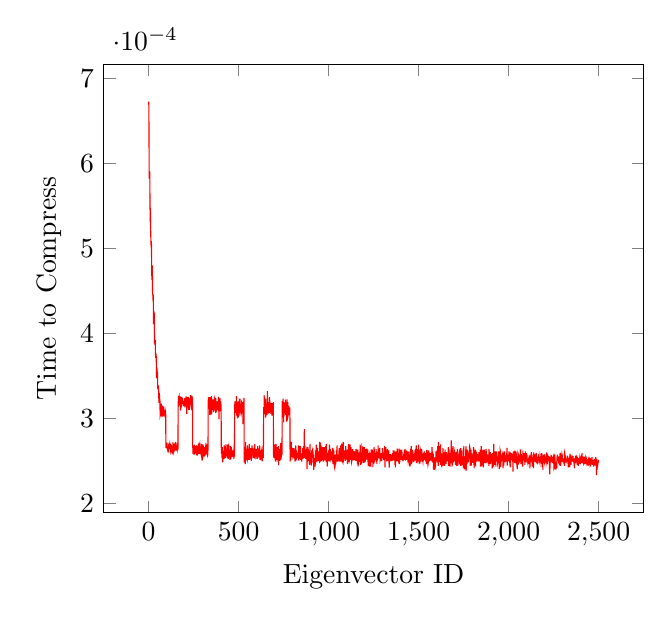
\begin{tikzpicture}
\begin{axis} [xlabel=Eigenvector ID, ylabel=Time to Compress]
\addplot[color=red] coordinates {
(1, 0.0006730556490000)
(2, 0.0006480216980000)
(3, 0.0005929470060000)
(4, 0.0005819797520000)
(5, 0.0005860328670000)
(6, 0.0005910396580000)
(7, 0.0005819797520000)
(8, 0.0005471706390000)
(9, 0.0005309581760000)
(10, 0.0005478858950000)
(11, 0.0005309581760000)
(12, 0.0005149841310000)
(13, 0.0005090236660000)
(14, 0.0005011558530000)
(15, 0.0005090236660000)
(16, 0.0005040168760000)
(17, 0.0004708766940000)
(18, 0.0004670619960000)
(19, 0.0004630088810000)
(20, 0.0004699230190000)
(21, 0.0004801750180000)
(22, 0.0004479885100000)
(23, 0.0004458427430000)
(24, 0.0004470348360000)
(25, 0.0004370212550000)
(26, 0.0004448890690000)
(27, 0.0004107952120000)
(28, 0.0004169940950000)
(29, 0.0004260540010000)
(30, 0.0004189014430000)
(31, 0.0004248619080000)
(32, 0.0004158020020000)
(33, 0.0003881454470000)
(34, 0.0003929138180000)
(35, 0.0003879070280000)
(36, 0.0003881454470000)
(37, 0.0003919601440000)
(38, 0.0003740787510000)
(39, 0.0003778934480000)
(40, 0.0003709793090000)
(41, 0.0003759860990000)
(42, 0.0003659725190000)
(43, 0.0003731250760000)
(44, 0.0003471374510000)
(45, 0.0003490448000000)
(46, 0.0003600120540000)
(47, 0.0003559589390000)
(48, 0.0003521442410000)
(49, 0.0003550052640000)
(50, 0.0003449916840000)
(51, 0.0003349781040000)
(52, 0.0003390312190000)
(53, 0.0003359317780000)
(54, 0.0003330707550000)
(55, 0.0003380775450000)
(56, 0.0003340244290000)
(57, 0.0003180503850000)
(58, 0.0003268718720000)
(59, 0.0003240108490000)
(60, 0.0003299713130000)
(61, 0.0003190040590000)
(62, 0.0003209114070000)
(63, 0.0003211498260000)
(64, 0.0003030300140000)
(65, 0.0003039836880000)
(66, 0.0003118515010000)
(67, 0.0003080368040000)
(68, 0.0003061294560000)
(69, 0.0003130435940000)
(70, 0.0003099441530000)
(71, 0.0003170967100000)
(72, 0.0003018379210000)
(73, 0.0003099441530000)
(74, 0.0003120899200000)
(75, 0.0003108978270000)
(76, 0.0003051757810000)
(77, 0.0003149509430000)
(78, 0.0003077983860000)
(79, 0.0003120899200000)
(80, 0.0003018379210000)
(81, 0.0003139972690000)
(82, 0.0003070831300000)
(83, 0.0003130435940000)
(84, 0.0003068447110000)
(85, 0.0003030300140000)
(86, 0.0003061294560000)
(87, 0.0003030300140000)
(88, 0.0003049373630000)
(89, 0.0003049373630000)
(90, 0.0003099441530000)
(91, 0.0003042221070000)
(92, 0.0003049373630000)
(93, 0.0003089904790000)
(94, 0.0003080368040000)
(95, 0.0003039836880000)
(96, 0.0002651214600000)
(97, 0.0002720355990000)
(98, 0.0002689361570000)
(99, 0.0002651214600000)
(100, 0.0002651214600000)
(101, 0.0002658367160000)
(102, 0.0002710819240000)
(103, 0.0002658367160000)
(104, 0.0002651214600000)
(105, 0.0002639293670000)
(106, 0.0002648830410000)
(107, 0.0002670288090000)
(108, 0.0002639293670000)
(109, 0.0002651214600000)
(110, 0.0002639293670000)
(111, 0.0002629756930000)
(112, 0.0002701282500000)
(113, 0.0002648830410000)
(114, 0.0002670288090000)
(115, 0.0002639293670000)
(116, 0.0002689361570000)
(117, 0.0002698898320000)
(118, 0.0002658367160000)
(119, 0.0002648830410000)
(120, 0.0002641677860000)
(121, 0.0002701282500000)
(122, 0.0002648830410000)
(123, 0.0002610683440000)
(124, 0.0002620220180000)
(125, 0.0002660751340000)
(126, 0.0002689361570000)
(127, 0.0002608299260000)
(128, 0.0002610683440000)
(129, 0.0002658367160000)
(130, 0.0002641677860000)
(131, 0.0002648830410000)
(132, 0.0002610683440000)
(133, 0.0002617836000000)
(134, 0.0002608299260000)
(135, 0.0002720355990000)
(136, 0.0002629756930000)
(137, 0.0002641677860000)
(138, 0.0002601146700000)
(139, 0.0002610683440000)
(140, 0.0002701282500000)
(141, 0.0002648830410000)
(142, 0.0002639293670000)
(143, 0.0002651214600000)
(144, 0.0002610683440000)
(145, 0.0002689361570000)
(146, 0.0002648830410000)
(147, 0.0002629756930000)
(148, 0.0002629756930000)
(149, 0.0002689361570000)
(150, 0.0002720355990000)
(151, 0.0002620220180000)
(152, 0.0002639293670000)
(153, 0.0002641677860000)
(154, 0.0002648830410000)
(155, 0.0002641677860000)
(156, 0.0002620220180000)
(157, 0.0002651214600000)
(158, 0.0002639293670000)
(159, 0.0002710819240000)
(160, 0.0002629756930000)
(161, 0.0002648830410000)
(162, 0.0002629756930000)
(163, 0.0002629756930000)
(164, 0.0003101825710000)
(165, 0.0003199577330000)
(166, 0.0003190040590000)
(167, 0.0003259181980000)
(168, 0.0003180503850000)
(169, 0.0003249645230000)
(170, 0.0003259181980000)
(171, 0.0003230571750000)
(172, 0.0003190040590000)
(173, 0.0003199577330000)
(174, 0.0003180503850000)
(175, 0.0003261566160000)
(176, 0.0003180503850000)
(177, 0.0003151893620000)
(178, 0.0003089904790000)
(179, 0.0003249645230000)
(180, 0.0003199577330000)
(181, 0.0003199577330000)
(182, 0.0003199577330000)
(183, 0.0003230571750000)
(184, 0.0003249645230000)
(185, 0.0003178119660000)
(186, 0.0003190040590000)
(187, 0.0003230571750000)
(188, 0.0003230571750000)
(189, 0.0003201961520000)
(190, 0.0003190040590000)
(191, 0.0003170967100000)
(192, 0.0003201961520000)
(193, 0.0003180503850000)
(194, 0.0003139972690000)
(195, 0.0003190040590000)
(196, 0.0003151893620000)
(197, 0.0003190040590000)
(198, 0.0003190040590000)
(199, 0.0003161430360000)
(200, 0.0003237724300000)
(201, 0.0003190040590000)
(202, 0.0003128051760000)
(203, 0.0003180503850000)
(204, 0.0003221035000000)
(205, 0.0003201961520000)
(206, 0.0003149509430000)
(207, 0.0003190040590000)
(208, 0.0003249645230000)
(209, 0.0003249645230000)
(210, 0.0003170967100000)
(211, 0.0003199577330000)
(212, 0.0003049373630000)
(213, 0.0003249645230000)
(214, 0.0003180503850000)
(215, 0.0003199577330000)
(216, 0.0003168582920000)
(217, 0.0003230571750000)
(218, 0.0003161430360000)
(219, 0.0003149509430000)
(220, 0.0003190040590000)
(221, 0.0003249645230000)
(222, 0.0003180503850000)
(223, 0.0003120899200000)
(224, 0.0003178119660000)
(225, 0.0003221035000000)
(226, 0.0003099441530000)
(227, 0.0003230571750000)
(228, 0.0003199577330000)
(229, 0.0003170967100000)
(230, 0.0003240108490000)
(231, 0.0003168582920000)
(232, 0.0003168582920000)
(233, 0.0003190040590000)
(234, 0.0003271102910000)
(235, 0.0003149509430000)
(236, 0.0003139972690000)
(237, 0.0003190040590000)
(238, 0.0003209114070000)
(239, 0.0003159046170000)
(240, 0.0003159046170000)
(241, 0.0003139972690000)
(242, 0.0003261566160000)
(243, 0.0003170967100000)
(244, 0.0003170967100000)
(245, 0.0002660751340000)
(246, 0.0002641677860000)
(247, 0.0002579689030000)
(248, 0.0002608299260000)
(249, 0.0002679824830000)
(250, 0.0002648830410000)
(251, 0.0002639293670000)
(252, 0.0002570152280000)
(253, 0.0002608299260000)
(254, 0.0002689361570000)
(255, 0.0002660751340000)
(256, 0.0002629756930000)
(257, 0.0002579689030000)
(258, 0.0002670288090000)
(259, 0.0002658367160000)
(260, 0.0002610683440000)
(261, 0.0002648830410000)
(262, 0.0002589225770000)
(263, 0.0002629756930000)
(264, 0.0002679824830000)
(265, 0.0002651214600000)
(266, 0.0002570152280000)
(267, 0.0002570152280000)
(268, 0.0002651214600000)
(269, 0.0002658367160000)
(270, 0.0002641677860000)
(271, 0.0002558231350000)
(272, 0.0002670288090000)
(273, 0.0002629756930000)
(274, 0.0002670288090000)
(275, 0.0002620220180000)
(276, 0.0002579689030000)
(277, 0.0002620220180000)
(278, 0.0002589225770000)
(279, 0.0002708435060000)
(280, 0.0002589225770000)
(281, 0.0002648830410000)
(282, 0.0002579689030000)
(283, 0.0002682209010000)
(284, 0.0002691745760000)
(285, 0.0002579689030000)
(286, 0.0002648830410000)
(287, 0.0002610683440000)
(288, 0.0002658367160000)
(289, 0.0002608299260000)
(290, 0.0002641677860000)
(291, 0.0002579689030000)
(292, 0.0002570152280000)
(293, 0.0002698898320000)
(294, 0.0002641677860000)
(295, 0.0002591609950000)
(296, 0.0002632141110000)
(297, 0.0002501010890000)
(298, 0.0002691745760000)
(299, 0.0002510547640000)
(300, 0.0002620220180000)
(301, 0.0002598762510000)
(302, 0.0002589225770000)
(303, 0.0002691745760000)
(304, 0.0002620220180000)
(305, 0.0002632141110000)
(306, 0.0002632141110000)
(307, 0.0002620220180000)
(308, 0.0002620220180000)
(309, 0.0002551078800000)
(310, 0.0002639293670000)
(311, 0.0002548694610000)
(312, 0.0002660751340000)
(313, 0.0002620220180000)
(314, 0.0002558231350000)
(315, 0.0002629756930000)
(316, 0.0002639293670000)
(317, 0.0002570152280000)
(318, 0.0002710819240000)
(319, 0.0002608299260000)
(320, 0.0002620220180000)
(321, 0.0002601146700000)
(322, 0.0002679824830000)
(323, 0.0002691745760000)
(324, 0.0002589225770000)
(325, 0.0002579689030000)
(326, 0.0002648830410000)
(327, 0.0002579689030000)
(328, 0.0002548694610000)
(329, 0.0002601146700000)
(330, 0.0002629756930000)
(331, 0.0003209114070000)
(332, 0.0003139972690000)
(333, 0.0003249645230000)
(334, 0.0003139972690000)
(335, 0.0003149509430000)
(336, 0.0003180503850000)
(337, 0.0003190040590000)
(338, 0.0003168582920000)
(339, 0.0003120899200000)
(340, 0.0003039836880000)
(341, 0.0003249645230000)
(342, 0.0003080368040000)
(343, 0.0003130435940000)
(344, 0.0003161430360000)
(345, 0.0003190040590000)
(346, 0.0003120899200000)
(347, 0.0003042221070000)
(348, 0.0003149509430000)
(349, 0.0003259181980000)
(350, 0.0003049373630000)
(351, 0.0003159046170000)
(352, 0.0003120899200000)
(353, 0.0003209114070000)
(354, 0.0003209114070000)
(355, 0.0003151893620000)
(356, 0.0003149509430000)
(357, 0.0003099441530000)
(358, 0.0003221035000000)
(359, 0.0003190040590000)
(360, 0.0003070831300000)
(361, 0.0003120899200000)
(362, 0.0003190040590000)
(363, 0.0003161430360000)
(364, 0.0003149509430000)
(365, 0.0003139972690000)
(366, 0.0003230571750000)
(367, 0.0003221035000000)
(368, 0.0003168582920000)
(369, 0.0003139972690000)
(370, 0.0003111362460000)
(371, 0.0003240108490000)
(372, 0.0003061294560000)
(373, 0.0003230571750000)
(374, 0.0003170967100000)
(375, 0.0003068447110000)
(376, 0.0003099441530000)
(377, 0.0003108978270000)
(378, 0.0003080368040000)
(379, 0.0003199577330000)
(380, 0.0003178119660000)
(381, 0.0003159046170000)
(382, 0.0003099441530000)
(383, 0.0003199577330000)
(384, 0.0003168582920000)
(385, 0.0003139972690000)
(386, 0.0003139972690000)
(387, 0.0003118515010000)
(388, 0.0003252029420000)
(389, 0.0003080368040000)
(390, 0.0003168582920000)
(391, 0.0002989768980000)
(392, 0.0003240108490000)
(393, 0.0003099441530000)
(394, 0.0003108978270000)
(395, 0.0003168582920000)
(396, 0.0003218650820000)
(397, 0.0003221035000000)
(398, 0.0003180503850000)
(399, 0.0003080368040000)
(400, 0.0003159046170000)
(401, 0.0003199577330000)
(402, 0.0003159046170000)
(403, 0.0003108978270000)
(404, 0.0002579689030000)
(405, 0.0002639293670000)
(406, 0.0002660751340000)
(407, 0.0002639293670000)
(408, 0.0002529621120000)
(409, 0.0002658367160000)
(410, 0.0002579689030000)
(411, 0.0002601146700000)
(412, 0.0002479553220000)
(413, 0.0002579689030000)
(414, 0.0002610683440000)
(415, 0.0002610683440000)
(416, 0.0002610683440000)
(417, 0.0002589225770000)
(418, 0.0002591609950000)
(419, 0.0002517700200000)
(420, 0.0002679824830000)
(421, 0.0002570152280000)
(422, 0.0002620220180000)
(423, 0.0002601146700000)
(424, 0.0002591609950000)
(425, 0.0002670288090000)
(426, 0.0002579689030000)
(427, 0.0002529621120000)
(428, 0.0002579689030000)
(429, 0.0002539157870000)
(430, 0.0002691745760000)
(431, 0.0002617836000000)
(432, 0.0002551078800000)
(433, 0.0002641677860000)
(434, 0.0002560615540000)
(435, 0.0002620220180000)
(436, 0.0002560615540000)
(437, 0.0002579689030000)
(438, 0.0002579689030000)
(439, 0.0002529621120000)
(440, 0.0002691745760000)
(441, 0.0002610683440000)
(442, 0.0002539157870000)
(443, 0.0002520084380000)
(444, 0.0002660751340000)
(445, 0.0002670288090000)
(446, 0.0002539157870000)
(447, 0.0002629756930000)
(448, 0.0002558231350000)
(449, 0.0002601146700000)
(450, 0.0002579689030000)
(451, 0.0002620220180000)
(452, 0.0002508163450000)
(453, 0.0002589225770000)
(454, 0.0002608299260000)
(455, 0.0002670288090000)
(456, 0.0002520084380000)
(457, 0.0002551078800000)
(458, 0.0002629756930000)
(459, 0.0002610683440000)
(460, 0.0002658367160000)
(461, 0.0002570152280000)
(462, 0.0002539157870000)
(463, 0.0002620220180000)
(464, 0.0002591609950000)
(465, 0.0002589225770000)
(466, 0.0002570152280000)
(467, 0.0002610683440000)
(468, 0.0002548694610000)
(469, 0.0002598762510000)
(470, 0.0002620220180000)
(471, 0.0002541542050000)
(472, 0.0002582073210000)
(473, 0.0002620220180000)
(474, 0.0002520084380000)
(475, 0.0002691745760000)
(476, 0.0002691745760000)
(477, 0.0002551078800000)
(478, 0.0003130435940000)
(479, 0.0003170967100000)
(480, 0.0003199577330000)
(481, 0.0003058910370000)
(482, 0.0003180503850000)
(483, 0.0003139972690000)
(484, 0.0003130435940000)
(485, 0.0003080368040000)
(486, 0.0003108978270000)
(487, 0.0003151893620000)
(488, 0.0003259181980000)
(489, 0.0003030300140000)
(490, 0.0003151893620000)
(491, 0.0003111362460000)
(492, 0.0003199577330000)
(493, 0.0003130435940000)
(494, 0.0002999305730000)
(495, 0.0003058910370000)
(496, 0.0003159046170000)
(497, 0.0003042221070000)
(498, 0.0003011226650000)
(499, 0.0003130435940000)
(500, 0.0003199577330000)
(501, 0.0003070831300000)
(502, 0.0003070831300000)
(503, 0.0003118515010000)
(504, 0.0003061294560000)
(505, 0.0003230571750000)
(506, 0.0003209114070000)
(507, 0.0003030300140000)
(508, 0.0003230571750000)
(509, 0.0003149509430000)
(510, 0.0003101825710000)
(511, 0.0003118515010000)
(512, 0.0003139972690000)
(513, 0.0003130435940000)
(514, 0.0003080368040000)
(515, 0.0003068447110000)
(516, 0.0003099441530000)
(517, 0.0003209114070000)
(518, 0.0003061294560000)
(519, 0.0003190040590000)
(520, 0.0003070831300000)
(521, 0.0003180503850000)
(522, 0.0003130435940000)
(523, 0.0003139972690000)
(524, 0.0002930164340000)
(525, 0.0003170967100000)
(526, 0.0003190040590000)
(527, 0.0003130435940000)
(528, 0.0003080368040000)
(529, 0.0003058910370000)
(530, 0.0003240108490000)
(531, 0.0002479553220000)
(532, 0.0002620220180000)
(533, 0.0002617836000000)
(534, 0.0002558231350000)
(535, 0.0002601146700000)
(536, 0.0002541542050000)
(537, 0.0002460479740000)
(538, 0.0002589225770000)
(539, 0.0002720355990000)
(540, 0.0002501010890000)
(541, 0.0002639293670000)
(542, 0.0002510547640000)
(543, 0.0002608299260000)
(544, 0.0002608299260000)
(545, 0.0002510547640000)
(546, 0.0002579689030000)
(547, 0.0002639293670000)
(548, 0.0002548694610000)
(549, 0.0002679824830000)
(550, 0.0002520084380000)
(551, 0.0002529621120000)
(552, 0.0002639293670000)
(553, 0.0002610683440000)
(554, 0.0002610683440000)
(555, 0.0002610683440000)
(556, 0.0002579689030000)
(557, 0.0002610683440000)
(558, 0.0002510547640000)
(559, 0.0002698898320000)
(560, 0.0002541542050000)
(561, 0.0002610683440000)
(562, 0.0002551078800000)
(563, 0.0002579689030000)
(564, 0.0002601146700000)
(565, 0.0002541542050000)
(566, 0.0002548694610000)
(567, 0.0002648830410000)
(568, 0.0002541542050000)
(569, 0.0002598762510000)
(570, 0.0002620220180000)
(571, 0.0002498626710000)
(572, 0.0002570152280000)
(573, 0.0002529621120000)
(574, 0.0002679824830000)
(575, 0.0002629756930000)
(576, 0.0002579689030000)
(577, 0.0002579689030000)
(578, 0.0002579689030000)
(579, 0.0002608299260000)
(580, 0.0002651214600000)
(581, 0.0002560615540000)
(582, 0.0002629756930000)
(583, 0.0002529621120000)
(584, 0.0002570152280000)
(585, 0.0002589225770000)
(586, 0.0002598762510000)
(587, 0.0002548694610000)
(588, 0.0002639293670000)
(589, 0.0002560615540000)
(590, 0.0002698898320000)
(591, 0.0002532005310000)
(592, 0.0002529621120000)
(593, 0.0002639293670000)
(594, 0.0002548694610000)
(595, 0.0002632141110000)
(596, 0.0002601146700000)
(597, 0.0002639293670000)
(598, 0.0002620220180000)
(599, 0.0002589225770000)
(600, 0.0002560615540000)
(601, 0.0002589225770000)
(602, 0.0002520084380000)
(603, 0.0002598762510000)
(604, 0.0002591609950000)
(605, 0.0002520084380000)
(606, 0.0002670288090000)
(607, 0.0002570152280000)
(608, 0.0002560615540000)
(609, 0.0002539157870000)
(610, 0.0002617836000000)
(611, 0.0002639293670000)
(612, 0.0002639293670000)
(613, 0.0002620220180000)
(614, 0.0002570152280000)
(615, 0.0002539157870000)
(616, 0.0002570152280000)
(617, 0.0002679824830000)
(618, 0.0002598762510000)
(619, 0.0002510547640000)
(620, 0.0002529621120000)
(621, 0.0002591609950000)
(622, 0.0002620220180000)
(623, 0.0002539157870000)
(624, 0.0002529621120000)
(625, 0.0002539157870000)
(626, 0.0002591609950000)
(627, 0.0002591609950000)
(628, 0.0002620220180000)
(629, 0.0002629756930000)
(630, 0.0002579689030000)
(631, 0.0002491474150000)
(632, 0.0002629756930000)
(633, 0.0002589225770000)
(634, 0.0002610683440000)
(635, 0.0002539157870000)
(636, 0.0002560615540000)
(637, 0.0002532005310000)
(638, 0.0002679824830000)
(639, 0.0003130435940000)
(640, 0.0003008842470000)
(641, 0.0003058910370000)
(642, 0.0003271102910000)
(643, 0.0003139972690000)
(644, 0.0003149509430000)
(645, 0.0003170967100000)
(646, 0.0003139972690000)
(647, 0.0003159046170000)
(648, 0.0003051757810000)
(649, 0.0003230571750000)
(650, 0.0003011226650000)
(651, 0.0003230571750000)
(652, 0.0003089904790000)
(653, 0.0003049373630000)
(654, 0.0003061294560000)
(655, 0.0003139972690000)
(656, 0.0003170967100000)
(657, 0.0003108978270000)
(658, 0.0003039836880000)
(659, 0.0003080368040000)
(660, 0.0003318786620000)
(661, 0.0003080368040000)
(662, 0.0003061294560000)
(663, 0.0003190040590000)
(664, 0.0003130435940000)
(665, 0.0003089904790000)
(666, 0.0003058910370000)
(667, 0.0003190040590000)
(668, 0.0003108978270000)
(669, 0.0003120899200000)
(670, 0.0003058910370000)
(671, 0.0003168582920000)
(672, 0.0003249645230000)
(673, 0.0003190040590000)
(674, 0.0003130435940000)
(675, 0.0003080368040000)
(676, 0.0003170967100000)
(677, 0.0003168582920000)
(678, 0.0003161430360000)
(679, 0.0003051757810000)
(680, 0.0003180503850000)
(681, 0.0003130435940000)
(682, 0.0003061294560000)
(683, 0.0003178119660000)
(684, 0.0003080368040000)
(685, 0.0003030300140000)
(686, 0.0003178119660000)
(687, 0.0003049373630000)
(688, 0.0003030300140000)
(689, 0.0003068447110000)
(690, 0.0003118515010000)
(691, 0.0003070831300000)
(692, 0.0003061294560000)
(693, 0.0003190040590000)
(694, 0.0002570152280000)
(695, 0.0002539157870000)
(696, 0.0002620220180000)
(697, 0.0002579689030000)
(698, 0.0002529621120000)
(699, 0.0002598762510000)
(700, 0.0002558231350000)
(701, 0.0002691745760000)
(702, 0.0002620220180000)
(703, 0.0002541542050000)
(704, 0.0002548694610000)
(705, 0.0002608299260000)
(706, 0.0002489089970000)
(707, 0.0002598762510000)
(708, 0.0002698898320000)
(709, 0.0002541542050000)
(710, 0.0002510547640000)
(711, 0.0002620220180000)
(712, 0.0002529621120000)
(713, 0.0002570152280000)
(714, 0.0002660751340000)
(715, 0.0002508163450000)
(716, 0.0002589225770000)
(717, 0.0002520084380000)
(718, 0.0002510547640000)
(719, 0.0002520084380000)
(720, 0.0002639293670000)
(721, 0.0002670288090000)
(722, 0.0002448558810000)
(723, 0.0002567768100000)
(724, 0.0002539157870000)
(725, 0.0002591609950000)
(726, 0.0002589225770000)
(727, 0.0002610683440000)
(728, 0.0002639293670000)
(729, 0.0002498626710000)
(730, 0.0002529621120000)
(731, 0.0002629756930000)
(732, 0.0002551078800000)
(733, 0.0002508163450000)
(734, 0.0002710819240000)
(735, 0.0002510547640000)
(736, 0.0002598762510000)
(737, 0.0002539157870000)
(738, 0.0002610683440000)
(739, 0.0002560615540000)
(740, 0.0002651214600000)
(741, 0.0002570152280000)
(742, 0.0003201961520000)
(743, 0.0003077983860000)
(744, 0.0003118515010000)
(745, 0.0003118515010000)
(746, 0.0003149509430000)
(747, 0.0003230571750000)
(748, 0.0003170967100000)
(749, 0.0003120899200000)
(750, 0.0002951622010000)
(751, 0.0003099441530000)
(752, 0.0003070831300000)
(753, 0.0003030300140000)
(754, 0.0003187656400000)
(755, 0.0003130435940000)
(756, 0.0003070831300000)
(757, 0.0003170967100000)
(758, 0.0003070831300000)
(759, 0.0003058910370000)
(760, 0.0003218650820000)
(761, 0.0003039836880000)
(762, 0.0003118515010000)
(763, 0.0003039836880000)
(764, 0.0003180503850000)
(765, 0.0003080368040000)
(766, 0.0002958774570000)
(767, 0.0003011226650000)
(768, 0.0003130435940000)
(769, 0.0003221035000000)
(770, 0.0003099441530000)
(771, 0.0003089904790000)
(772, 0.0003049373630000)
(773, 0.0003190040590000)
(774, 0.0003020763400000)
(775, 0.0003030300140000)
(776, 0.0003149509430000)
(777, 0.0003118515010000)
(778, 0.0003089904790000)
(779, 0.0003149509430000)
(780, 0.0003108978270000)
(781, 0.0003039836880000)
(782, 0.0003108978270000)
(783, 0.0003120899200000)
(784, 0.0003120899200000)
(785, 0.0003101825710000)
(786, 0.0002489089970000)
(787, 0.0002579689030000)
(788, 0.0002579689030000)
(789, 0.0002501010890000)
(790, 0.0002532005310000)
(791, 0.0002558231350000)
(792, 0.0002582073210000)
(793, 0.0002720355990000)
(794, 0.0002589225770000)
(795, 0.0002570152280000)
(796, 0.0002608299260000)
(797, 0.0002598762510000)
(798, 0.0002548694610000)
(799, 0.0002548694610000)
(800, 0.0002651214600000)
(801, 0.0002570152280000)
(802, 0.0002582073210000)
(803, 0.0002570152280000)
(804, 0.0002548694610000)
(805, 0.0002551078800000)
(806, 0.0002608299260000)
(807, 0.0002551078800000)
(808, 0.0002648830410000)
(809, 0.0002520084380000)
(810, 0.0002551078800000)
(811, 0.0002629756930000)
(812, 0.0002579689030000)
(813, 0.0002510547640000)
(814, 0.0002489089970000)
(815, 0.0002520084380000)
(816, 0.0002601146700000)
(817, 0.0002679824830000)
(818, 0.0002589225770000)
(819, 0.0002579689030000)
(820, 0.0002539157870000)
(821, 0.0002532005310000)
(822, 0.0002610683440000)
(823, 0.0002539157870000)
(824, 0.0002579689030000)
(825, 0.0002570152280000)
(826, 0.0002570152280000)
(827, 0.0002529621120000)
(828, 0.0002560615540000)
(829, 0.0002579689030000)
(830, 0.0002551078800000)
(831, 0.0002589225770000)
(832, 0.0002520084380000)
(833, 0.0002679824830000)
(834, 0.0002501010890000)
(835, 0.0002629756930000)
(836, 0.0002570152280000)
(837, 0.0002532005310000)
(838, 0.0002579689030000)
(839, 0.0002670288090000)
(840, 0.0002520084380000)
(841, 0.0002620220180000)
(842, 0.0002529621120000)
(843, 0.0002610683440000)
(844, 0.0002670288090000)
(845, 0.0002510547640000)
(846, 0.0002560615540000)
(847, 0.0002579689030000)
(848, 0.0002579689030000)
(849, 0.0002560615540000)
(850, 0.0002579689030000)
(851, 0.0002489089970000)
(852, 0.0002570152280000)
(853, 0.0002529621120000)
(854, 0.0002529621120000)
(855, 0.0002570152280000)
(856, 0.0002648830410000)
(857, 0.0002570152280000)
(858, 0.0002520084380000)
(859, 0.0002620220180000)
(860, 0.0002551078800000)
(861, 0.0002670288090000)
(862, 0.0002560615540000)
(863, 0.0002641677860000)
(864, 0.0002551078800000)
(865, 0.0002870559690000)
(866, 0.0002532005310000)
(867, 0.0002570152280000)
(868, 0.0002679824830000)
(869, 0.0002579689030000)
(870, 0.0002620220180000)
(871, 0.0002560615540000)
(872, 0.0002520084380000)
(873, 0.0002591609950000)
(874, 0.0002560615540000)
(875, 0.0002529621120000)
(876, 0.0002589225770000)
(877, 0.0002620220180000)
(878, 0.0002608299260000)
(879, 0.0002510547640000)
(880, 0.0002400875090000)
(881, 0.0002629756930000)
(882, 0.0002481937410000)
(883, 0.0002560615540000)
(884, 0.0002658367160000)
(885, 0.0002520084380000)
(886, 0.0002520084380000)
(887, 0.0002629756930000)
(888, 0.0002498626710000)
(889, 0.0002570152280000)
(890, 0.0002598762510000)
(891, 0.0002589225770000)
(892, 0.0002489089970000)
(893, 0.0002501010890000)
(894, 0.0002460479740000)
(895, 0.0002448558810000)
(896, 0.0002582073210000)
(897, 0.0002698898320000)
(898, 0.0002520084380000)
(899, 0.0002589225770000)
(900, 0.0002520084380000)
(901, 0.0002548694610000)
(902, 0.0002529621120000)
(903, 0.0002570152280000)
(904, 0.0002441406250000)
(905, 0.0002481937410000)
(906, 0.0002620220180000)
(907, 0.0002548694610000)
(908, 0.0002579689030000)
(909, 0.0002610683440000)
(910, 0.0002529621120000)
(911, 0.0002601146700000)
(912, 0.0002589225770000)
(913, 0.0002601146700000)
(914, 0.0002570152280000)
(915, 0.0002470016480000)
(916, 0.0002570152280000)
(917, 0.0002391338350000)
(918, 0.0002429485320000)
(919, 0.0002479553220000)
(920, 0.0002489089970000)
(921, 0.0002529621120000)
(922, 0.0002489089970000)
(923, 0.0002520084380000)
(924, 0.0002470016480000)
(925, 0.0002429485320000)
(926, 0.0002501010890000)
(927, 0.0002620220180000)
(928, 0.0002598762510000)
(929, 0.0002520084380000)
(930, 0.0002491474150000)
(931, 0.0002689361570000)
(932, 0.0002510547640000)
(933, 0.0002491474150000)
(934, 0.0002541542050000)
(935, 0.0002479553220000)
(936, 0.0002570152280000)
(937, 0.0002520084380000)
(938, 0.0002560615540000)
(939, 0.0002648830410000)
(940, 0.0002529621120000)
(941, 0.0002558231350000)
(942, 0.0002498626710000)
(943, 0.0002570152280000)
(944, 0.0002610683440000)
(945, 0.0002520084380000)
(946, 0.0002539157870000)
(947, 0.0002589225770000)
(948, 0.0002601146700000)
(949, 0.0002501010890000)
(950, 0.0002470016480000)
(951, 0.0002720355990000)
(952, 0.0002489089970000)
(953, 0.0002491474150000)
(954, 0.0002710819240000)
(955, 0.0002598762510000)
(956, 0.0002541542050000)
(957, 0.0002498626710000)
(958, 0.0002679824830000)
(959, 0.0002501010890000)
(960, 0.0002501010890000)
(961, 0.0002517700200000)
(962, 0.0002570152280000)
(963, 0.0002610683440000)
(964, 0.0002551078800000)
(965, 0.0002660751340000)
(966, 0.0002510547640000)
(967, 0.0002570152280000)
(968, 0.0002510547640000)
(969, 0.0002558231350000)
(970, 0.0002489089970000)
(971, 0.0002548694610000)
(972, 0.0002551078800000)
(973, 0.0002660751340000)
(974, 0.0002589225770000)
(975, 0.0002501010890000)
(976, 0.0002658367160000)
(977, 0.0002551078800000)
(978, 0.0002529621120000)
(979, 0.0002510547640000)
(980, 0.0002560615540000)
(981, 0.0002639293670000)
(982, 0.0002560615540000)
(983, 0.0002510547640000)
(984, 0.0002670288090000)
(985, 0.0002539157870000)
(986, 0.0002481937410000)
(987, 0.0002698898320000)
(988, 0.0002560615540000)
(989, 0.0002541542050000)
(990, 0.0002589225770000)
(991, 0.0002567768100000)
(992, 0.0002429485320000)
(993, 0.0002501010890000)
(994, 0.0002567768100000)
(995, 0.0002548694610000)
(996, 0.0002570152280000)
(997, 0.0002510547640000)
(998, 0.0002589225770000)
(999, 0.0002579689030000)
(1000, 0.0002501010890000)
(1001, 0.0002501010890000)
(1002, 0.0002551078800000)
(1003, 0.0002620220180000)
(1004, 0.0002489089970000)
(1005, 0.0002689361570000)
(1006, 0.0002620220180000)
(1007, 0.0002501010890000)
(1008, 0.0002591609950000)
(1009, 0.0002639293670000)
(1010, 0.0002598762510000)
(1011, 0.0002529621120000)
(1012, 0.0002539157870000)
(1013, 0.0002579689030000)
(1014, 0.0002608299260000)
(1015, 0.0002551078800000)
(1016, 0.0002570152280000)
(1017, 0.0002532005310000)
(1018, 0.0002539157870000)
(1019, 0.0002510547640000)
(1020, 0.0002539157870000)
(1021, 0.0002620220180000)
(1022, 0.0002489089970000)
(1023, 0.0002651214600000)
(1024, 0.0002460479740000)
(1025, 0.0002520084380000)
(1026, 0.0002551078800000)
(1027, 0.0002598762510000)
(1028, 0.0002629756930000)
(1029, 0.0002529621120000)
(1030, 0.0002539157870000)
(1031, 0.0002470016480000)
(1032, 0.0002429485320000)
(1033, 0.0002419948580000)
(1034, 0.0002498626710000)
(1035, 0.0002570152280000)
(1036, 0.0002419948580000)
(1037, 0.0002501010890000)
(1038, 0.0002470016480000)
(1039, 0.0002501010890000)
(1040, 0.0002491474150000)
(1041, 0.0002529621120000)
(1042, 0.0002520084380000)
(1043, 0.0002539157870000)
(1044, 0.0002620220180000)
(1045, 0.0002498626710000)
(1046, 0.0002570152280000)
(1047, 0.0002679824830000)
(1048, 0.0002489089970000)
(1049, 0.0002520084380000)
(1050, 0.0002529621120000)
(1051, 0.0002570152280000)
(1052, 0.0002501010890000)
(1053, 0.0002548694610000)
(1054, 0.0002548694610000)
(1055, 0.0002529621120000)
(1056, 0.0002541542050000)
(1057, 0.0002541542050000)
(1058, 0.0002620220180000)
(1059, 0.0002648830410000)
(1060, 0.0002489089970000)
(1061, 0.0002579689030000)
(1062, 0.0002570152280000)
(1063, 0.0002489089970000)
(1064, 0.0002620220180000)
(1065, 0.0002560615540000)
(1066, 0.0002589225770000)
(1067, 0.0002679824830000)
(1068, 0.0002498626710000)
(1069, 0.0002551078800000)
(1070, 0.0002579689030000)
(1071, 0.0002489089970000)
(1072, 0.0002529621120000)
(1073, 0.0002701282500000)
(1074, 0.0002532005310000)
(1075, 0.0002620220180000)
(1076, 0.0002510547640000)
(1077, 0.0002520084380000)
(1078, 0.0002510547640000)
(1079, 0.0002501010890000)
(1080, 0.0002560615540000)
(1081, 0.0002720355990000)
(1082, 0.0002479553220000)
(1083, 0.0002520084380000)
(1084, 0.0002570152280000)
(1085, 0.0002532005310000)
(1086, 0.0002620220180000)
(1087, 0.0002570152280000)
(1088, 0.0002620220180000)
(1089, 0.0002570152280000)
(1090, 0.0002520084380000)
(1091, 0.0002582073210000)
(1092, 0.0002520084380000)
(1093, 0.0002498626710000)
(1094, 0.0002539157870000)
(1095, 0.0002670288090000)
(1096, 0.0002620220180000)
(1097, 0.0002589225770000)
(1098, 0.0002520084380000)
(1099, 0.0002520084380000)
(1100, 0.0002529621120000)
(1101, 0.0002620220180000)
(1102, 0.0002579689030000)
(1103, 0.0002539157870000)
(1104, 0.0002629756930000)
(1105, 0.0002460479740000)
(1106, 0.0002548694610000)
(1107, 0.0002501010890000)
(1108, 0.0002639293670000)
(1109, 0.0002489089970000)
(1110, 0.0002491474150000)
(1111, 0.0002698898320000)
(1112, 0.0002520084380000)
(1113, 0.0002510547640000)
(1114, 0.0002560615540000)
(1115, 0.0002548694610000)
(1116, 0.0002629756930000)
(1117, 0.0002548694610000)
(1118, 0.0002510547640000)
(1119, 0.0002691745760000)
(1120, 0.0002579689030000)
(1121, 0.0002520084380000)
(1122, 0.0002539157870000)
(1123, 0.0002539157870000)
(1124, 0.0002660751340000)
(1125, 0.0002510547640000)
(1126, 0.0002570152280000)
(1127, 0.0002579689030000)
(1128, 0.0002489089970000)
(1129, 0.0002498626710000)
(1130, 0.0002570152280000)
(1131, 0.0002570152280000)
(1132, 0.0002532005310000)
(1133, 0.0002629756930000)
(1134, 0.0002629756930000)
(1135, 0.0002551078800000)
(1136, 0.0002510547640000)
(1137, 0.0002510547640000)
(1138, 0.0002610683440000)
(1139, 0.0002579689030000)
(1140, 0.0002541542050000)
(1141, 0.0002610683440000)
(1142, 0.0002510547640000)
(1143, 0.0002598762510000)
(1144, 0.0002598762510000)
(1145, 0.0002560615540000)
(1146, 0.0002608299260000)
(1147, 0.0002501010890000)
(1148, 0.0002610683440000)
(1149, 0.0002541542050000)
(1150, 0.0002501010890000)
(1151, 0.0002591609950000)
(1152, 0.0002639293670000)
(1153, 0.0002498626710000)
(1154, 0.0002570152280000)
(1155, 0.0002508163450000)
(1156, 0.0002598762510000)
(1157, 0.0002520084380000)
(1158, 0.0002501010890000)
(1159, 0.0002629756930000)
(1160, 0.0002501010890000)
(1161, 0.0002510547640000)
(1162, 0.0002629756930000)
(1163, 0.0002508163450000)
(1164, 0.0002429485320000)
(1165, 0.0002508163450000)
(1166, 0.0002560615540000)
(1167, 0.0002548694610000)
(1168, 0.0002598762510000)
(1169, 0.0002520084380000)
(1170, 0.0002510547640000)
(1171, 0.0002481937410000)
(1172, 0.0002520084380000)
(1173, 0.0002510547640000)
(1174, 0.0002498626710000)
(1175, 0.0002689361570000)
(1176, 0.0002617836000000)
(1177, 0.0002520084380000)
(1178, 0.0002450942990000)
(1179, 0.0002639293670000)
(1180, 0.0002648830410000)
(1181, 0.0002460479740000)
(1182, 0.0002548694610000)
(1183, 0.0002570152280000)
(1184, 0.0002598762510000)
(1185, 0.0002470016480000)
(1186, 0.0002529621120000)
(1187, 0.0002539157870000)
(1188, 0.0002498626710000)
(1189, 0.0002660751340000)
(1190, 0.0002660751340000)
(1191, 0.0002551078800000)
(1192, 0.0002589225770000)
(1193, 0.0002510547640000)
(1194, 0.0002589225770000)
(1195, 0.0002470016480000)
(1196, 0.0002570152280000)
(1197, 0.0002570152280000)
(1198, 0.0002658367160000)
(1199, 0.0002510547640000)
(1200, 0.0002551078800000)
(1201, 0.0002501010890000)
(1202, 0.0002501010890000)
(1203, 0.0002481937410000)
(1204, 0.0002558231350000)
(1205, 0.0002560615540000)
(1206, 0.0002639293670000)
(1207, 0.0002551078800000)
(1208, 0.0002529621120000)
(1209, 0.0002560615540000)
(1210, 0.0002551078800000)
(1211, 0.0002520084380000)
(1212, 0.0002520084380000)
(1213, 0.0002641677860000)
(1214, 0.0002539157870000)
(1215, 0.0002598762510000)
(1216, 0.0002529621120000)
(1217, 0.0002532005310000)
(1218, 0.0002629756930000)
(1219, 0.0002489089970000)
(1220, 0.0002498626710000)
(1221, 0.0002589225770000)
(1222, 0.0002501010890000)
(1223, 0.0002439022060000)
(1224, 0.0002479553220000)
(1225, 0.0002510547640000)
(1226, 0.0002498626710000)
(1227, 0.0002429485320000)
(1228, 0.0002558231350000)
(1229, 0.0002548694610000)
(1230, 0.0002560615540000)
(1231, 0.0002591609950000)
(1232, 0.0002501010890000)
(1233, 0.0002589225770000)
(1234, 0.0002429485320000)
(1235, 0.0002589225770000)
(1236, 0.0002589225770000)
(1237, 0.0002632141110000)
(1238, 0.0002479553220000)
(1239, 0.0002510547640000)
(1240, 0.0002491474150000)
(1241, 0.0002610683440000)
(1242, 0.0002539157870000)
(1243, 0.0002629756930000)
(1244, 0.0002541542050000)
(1245, 0.0002520084380000)
(1246, 0.0002419948580000)
(1247, 0.0002608299260000)
(1248, 0.0002529621120000)
(1249, 0.0002548694610000)
(1250, 0.0002510547640000)
(1251, 0.0002460479740000)
(1252, 0.0002639293670000)
(1253, 0.0002660751340000)
(1254, 0.0002479553220000)
(1255, 0.0002598762510000)
(1256, 0.0002489089970000)
(1257, 0.0002558231350000)
(1258, 0.0002551078800000)
(1259, 0.0002548694610000)
(1260, 0.0002558231350000)
(1261, 0.0002520084380000)
(1262, 0.0002517700200000)
(1263, 0.0002520084380000)
(1264, 0.0002639293670000)
(1265, 0.0002510547640000)
(1266, 0.0002589225770000)
(1267, 0.0002520084380000)
(1268, 0.0002460479740000)
(1269, 0.0002601146700000)
(1270, 0.0002551078800000)
(1271, 0.0002501010890000)
(1272, 0.0002529621120000)
(1273, 0.0002589225770000)
(1274, 0.0002529621120000)
(1275, 0.0002679824830000)
(1276, 0.0002570152280000)
(1277, 0.0002560615540000)
(1278, 0.0002579689030000)
(1279, 0.0002529621120000)
(1280, 0.0002560615540000)
(1281, 0.0002570152280000)
(1282, 0.0002539157870000)
(1283, 0.0002570152280000)
(1284, 0.0002651214600000)
(1285, 0.0002560615540000)
(1286, 0.0002501010890000)
(1287, 0.0002508163450000)
(1288, 0.0002529621120000)
(1289, 0.0002541542050000)
(1290, 0.0002529621120000)
(1291, 0.0002529621120000)
(1292, 0.0002589225770000)
(1293, 0.0002558231350000)
(1294, 0.0002498626710000)
(1295, 0.0002558231350000)
(1296, 0.0002589225770000)
(1297, 0.0002551078800000)
(1298, 0.0002570152280000)
(1299, 0.0002548694610000)
(1300, 0.0002648830410000)
(1301, 0.0002529621120000)
(1302, 0.0002579689030000)
(1303, 0.0002567768100000)
(1304, 0.0002529621120000)
(1305, 0.0002508163450000)
(1306, 0.0002579689030000)
(1307, 0.0002520084380000)
(1308, 0.0002582073210000)
(1309, 0.0002589225770000)
(1310, 0.0002560615540000)
(1311, 0.0002670288090000)
(1312, 0.0002510547640000)
(1313, 0.0002419948580000)
(1314, 0.0002579689030000)
(1315, 0.0002539157870000)
(1316, 0.0002570152280000)
(1317, 0.0002539157870000)
(1318, 0.0002660751340000)
(1319, 0.0002539157870000)
(1320, 0.0002520084380000)
(1321, 0.0002551078800000)
(1322, 0.0002620220180000)
(1323, 0.0002491474150000)
(1324, 0.0002620220180000)
(1325, 0.0002558231350000)
(1326, 0.0002548694610000)
(1327, 0.0002639293670000)
(1328, 0.0002601146700000)
(1329, 0.0002532005310000)
(1330, 0.0002520084380000)
(1331, 0.0002501010890000)
(1332, 0.0002608299260000)
(1333, 0.0002541542050000)
(1334, 0.0002620220180000)
(1335, 0.0002548694610000)
(1336, 0.0002431869510000)
(1337, 0.0002419948580000)
(1338, 0.0002520084380000)
(1339, 0.0002539157870000)
(1340, 0.0002558231350000)
(1341, 0.0002501010890000)
(1342, 0.0002570152280000)
(1343, 0.0002570152280000)
(1344, 0.0002548694610000)
(1345, 0.0002567768100000)
(1346, 0.0002508163450000)
(1347, 0.0002570152280000)
(1348, 0.0002529621120000)
(1349, 0.0002508163450000)
(1350, 0.0002510547640000)
(1351, 0.0002529621120000)
(1352, 0.0002548694610000)
(1353, 0.0002498626710000)
(1354, 0.0002589225770000)
(1355, 0.0002510547640000)
(1356, 0.0002548694610000)
(1357, 0.0002541542050000)
(1358, 0.0002501010890000)
(1359, 0.0002620220180000)
(1360, 0.0002510547640000)
(1361, 0.0002589225770000)
(1362, 0.0002591609950000)
(1363, 0.0002598762510000)
(1364, 0.0002620220180000)
(1365, 0.0002551078800000)
(1366, 0.0002510547640000)
(1367, 0.0002589225770000)
(1368, 0.0002450942990000)
(1369, 0.0002601146700000)
(1370, 0.0002579689030000)
(1371, 0.0002419948580000)
(1372, 0.0002501010890000)
(1373, 0.0002529621120000)
(1374, 0.0002608299260000)
(1375, 0.0002520084380000)
(1376, 0.0002539157870000)
(1377, 0.0002570152280000)
(1378, 0.0002491474150000)
(1379, 0.0002529621120000)
(1380, 0.0002539157870000)
(1381, 0.0002641677860000)
(1382, 0.0002570152280000)
(1383, 0.0002589225770000)
(1384, 0.0002491474150000)
(1385, 0.0002579689030000)
(1386, 0.0002520084380000)
(1387, 0.0002510547640000)
(1388, 0.0002582073210000)
(1389, 0.0002548694610000)
(1390, 0.0002560615540000)
(1391, 0.0002641677860000)
(1392, 0.0002460479740000)
(1393, 0.0002501010890000)
(1394, 0.0002510547640000)
(1395, 0.0002479553220000)
(1396, 0.0002601146700000)
(1397, 0.0002520084380000)
(1398, 0.0002558231350000)
(1399, 0.0002629756930000)
(1400, 0.0002539157870000)
(1401, 0.0002510547640000)
(1402, 0.0002589225770000)
(1403, 0.0002567768100000)
(1404, 0.0002520084380000)
(1405, 0.0002629756930000)
(1406, 0.0002510547640000)
(1407, 0.0002598762510000)
(1408, 0.0002598762510000)
(1409, 0.0002501010890000)
(1410, 0.0002520084380000)
(1411, 0.0002532005310000)
(1412, 0.0002539157870000)
(1413, 0.0002539157870000)
(1414, 0.0002491474150000)
(1415, 0.0002548694610000)
(1416, 0.0002548694610000)
(1417, 0.0002579689030000)
(1418, 0.0002539157870000)
(1419, 0.0002520084380000)
(1420, 0.0002579689030000)
(1421, 0.0002629756930000)
(1422, 0.0002508163450000)
(1423, 0.0002570152280000)
(1424, 0.0002539157870000)
(1425, 0.0002639293670000)
(1426, 0.0002589225770000)
(1427, 0.0002589225770000)
(1428, 0.0002501010890000)
(1429, 0.0002560615540000)
(1430, 0.0002548694610000)
(1431, 0.0002541542050000)
(1432, 0.0002510547640000)
(1433, 0.0002620220180000)
(1434, 0.0002548694610000)
(1435, 0.0002601146700000)
(1436, 0.0002539157870000)
(1437, 0.0002567768100000)
(1438, 0.0002548694610000)
(1439, 0.0002529621120000)
(1440, 0.0002551078800000)
(1441, 0.0002608299260000)
(1442, 0.0002558231350000)
(1443, 0.0002498626710000)
(1444, 0.0002510547640000)
(1445, 0.0002601146700000)
(1446, 0.0002539157870000)
(1447, 0.0002510547640000)
(1448, 0.0002498626710000)
(1449, 0.0002570152280000)
(1450, 0.0002431869510000)
(1451, 0.0002520084380000)
(1452, 0.0002529621120000)
(1453, 0.0002520084380000)
(1454, 0.0002570152280000)
(1455, 0.0002639293670000)
(1456, 0.0002479553220000)
(1457, 0.0002489089970000)
(1458, 0.0002560615540000)
(1459, 0.0002670288090000)
(1460, 0.0002460479740000)
(1461, 0.0002598762510000)
(1462, 0.0002560615540000)
(1463, 0.0002479553220000)
(1464, 0.0002629756930000)
(1465, 0.0002610683440000)
(1466, 0.0002579689030000)
(1467, 0.0002608299260000)
(1468, 0.0002539157870000)
(1469, 0.0002551078800000)
(1470, 0.0002539157870000)
(1471, 0.0002570152280000)
(1472, 0.0002529621120000)
(1473, 0.0002481937410000)
(1474, 0.0002560615540000)
(1475, 0.0002579689030000)
(1476, 0.0002541542050000)
(1477, 0.0002548694610000)
(1478, 0.0002510547640000)
(1479, 0.0002620220180000)
(1480, 0.0002501010890000)
(1481, 0.0002551078800000)
(1482, 0.0002579689030000)
(1483, 0.0002639293670000)
(1484, 0.0002501010890000)
(1485, 0.0002601146700000)
(1486, 0.0002601146700000)
(1487, 0.0002679824830000)
(1488, 0.0002470016480000)
(1489, 0.0002529621120000)
(1490, 0.0002639293670000)
(1491, 0.0002570152280000)
(1492, 0.0002541542050000)
(1493, 0.0002629756930000)
(1494, 0.0002510547640000)
(1495, 0.0002520084380000)
(1496, 0.0002517700200000)
(1497, 0.0002489089970000)
(1498, 0.0002598762510000)
(1499, 0.0002579689030000)
(1500, 0.0002689361570000)
(1501, 0.0002520084380000)
(1502, 0.0002501010890000)
(1503, 0.0002510547640000)
(1504, 0.0002548694610000)
(1505, 0.0002548694610000)
(1506, 0.0002517700200000)
(1507, 0.0002460479740000)
(1508, 0.0002598762510000)
(1509, 0.0002610683440000)
(1510, 0.0002551078800000)
(1511, 0.0002520084380000)
(1512, 0.0002529621120000)
(1513, 0.0002620220180000)
(1514, 0.0002489089970000)
(1515, 0.0002639293670000)
(1516, 0.0002510547640000)
(1517, 0.0002629756930000)
(1518, 0.0002570152280000)
(1519, 0.0002579689030000)
(1520, 0.0002560615540000)
(1521, 0.0002579689030000)
(1522, 0.0002489089970000)
(1523, 0.0002508163450000)
(1524, 0.0002491474150000)
(1525, 0.0002520084380000)
(1526, 0.0002532005310000)
(1527, 0.0002539157870000)
(1528, 0.0002589225770000)
(1529, 0.0002501010890000)
(1530, 0.0002601146700000)
(1531, 0.0002510547640000)
(1532, 0.0002608299260000)
(1533, 0.0002539157870000)
(1534, 0.0002560615540000)
(1535, 0.0002560615540000)
(1536, 0.0002570152280000)
(1537, 0.0002570152280000)
(1538, 0.0002591609950000)
(1539, 0.0002532005310000)
(1540, 0.0002489089970000)
(1541, 0.0002520084380000)
(1542, 0.0002560615540000)
(1543, 0.0002510547640000)
(1544, 0.0002460479740000)
(1545, 0.0002620220180000)
(1546, 0.0002620220180000)
(1547, 0.0002620220180000)
(1548, 0.0002560615540000)
(1549, 0.0002479553220000)
(1550, 0.0002498626710000)
(1551, 0.0002479553220000)
(1552, 0.0002450942990000)
(1553, 0.0002460479740000)
(1554, 0.0002579689030000)
(1555, 0.0002601146700000)
(1556, 0.0002610683440000)
(1557, 0.0002608299260000)
(1558, 0.0002570152280000)
(1559, 0.0002498626710000)
(1560, 0.0002501010890000)
(1561, 0.0002510547640000)
(1562, 0.0002589225770000)
(1563, 0.0002548694610000)
(1564, 0.0002508163450000)
(1565, 0.0002570152280000)
(1566, 0.0002548694610000)
(1567, 0.0002501010890000)
(1568, 0.0002529621120000)
(1569, 0.0002570152280000)
(1570, 0.0002598762510000)
(1571, 0.0002510547640000)
(1572, 0.0002510547640000)
(1573, 0.0002567768100000)
(1574, 0.0002658367160000)
(1575, 0.0002479553220000)
(1576, 0.0002610683440000)
(1577, 0.0002539157870000)
(1578, 0.0002551078800000)
(1579, 0.0002558231350000)
(1580, 0.0002510547640000)
(1581, 0.0002579689030000)
(1582, 0.0002398490910000)
(1583, 0.0002470016480000)
(1584, 0.0002481937410000)
(1585, 0.0002439022060000)
(1586, 0.0002510547640000)
(1587, 0.0002391338350000)
(1588, 0.0002429485320000)
(1589, 0.0002539157870000)
(1590, 0.0002501010890000)
(1591, 0.0002481937410000)
(1592, 0.0002458095550000)
(1593, 0.0002450942990000)
(1594, 0.0002439022060000)
(1595, 0.0002489089970000)
(1596, 0.0002610683440000)
(1597, 0.0002520084380000)
(1598, 0.0002529621120000)
(1599, 0.0002520084380000)
(1600, 0.0002501010890000)
(1601, 0.0002529621120000)
(1602, 0.0002620220180000)
(1603, 0.0002541542050000)
(1604, 0.0002479553220000)
(1605, 0.0002591609950000)
(1606, 0.0002670288090000)
(1607, 0.0002489089970000)
(1608, 0.0002667903900000)
(1609, 0.0002439022060000)
(1610, 0.0002720355990000)
(1611, 0.0002450942990000)
(1612, 0.0002539157870000)
(1613, 0.0002510547640000)
(1614, 0.0002620220180000)
(1615, 0.0002510547640000)
(1616, 0.0002481937410000)
(1617, 0.0002560615540000)
(1618, 0.0002670288090000)
(1619, 0.0002501010890000)
(1620, 0.0002501010890000)
(1621, 0.0002489089970000)
(1622, 0.0002691745760000)
(1623, 0.0002450942990000)
(1624, 0.0002589225770000)
(1625, 0.0002498626710000)
(1626, 0.0002510547640000)
(1627, 0.0002520084380000)
(1628, 0.0002460479740000)
(1629, 0.0002419948580000)
(1630, 0.0002558231350000)
(1631, 0.0002582073210000)
(1632, 0.0002532005310000)
(1633, 0.0002548694610000)
(1634, 0.0002489089970000)
(1635, 0.0002648830410000)
(1636, 0.0002441406250000)
(1637, 0.0002560615540000)
(1638, 0.0002489089970000)
(1639, 0.0002589225770000)
(1640, 0.0002548694610000)
(1641, 0.0002510547640000)
(1642, 0.0002498626710000)
(1643, 0.0002598762510000)
(1644, 0.0002439022060000)
(1645, 0.0002510547640000)
(1646, 0.0002539157870000)
(1647, 0.0002629756930000)
(1648, 0.0002520084380000)
(1649, 0.0002560615540000)
(1650, 0.0002560615540000)
(1651, 0.0002579689030000)
(1652, 0.0002460479740000)
(1653, 0.0002520084380000)
(1654, 0.0002601146700000)
(1655, 0.0002579689030000)
(1656, 0.0002520084380000)
(1657, 0.0002570152280000)
(1658, 0.0002510547640000)
(1659, 0.0002551078800000)
(1660, 0.0002491474150000)
(1661, 0.0002570152280000)
(1662, 0.0002520084380000)
(1663, 0.0002548694610000)
(1664, 0.0002610683440000)
(1665, 0.0002660751340000)
(1666, 0.0002439022060000)
(1667, 0.0002620220180000)
(1668, 0.0002460479740000)
(1669, 0.0002632141110000)
(1670, 0.0002529621120000)
(1671, 0.0002589225770000)
(1672, 0.0002460479740000)
(1673, 0.0002589225770000)
(1674, 0.0002429485320000)
(1675, 0.0002520084380000)
(1676, 0.0002491474150000)
(1677, 0.0002510547640000)
(1678, 0.0002520084380000)
(1679, 0.0002560615540000)
(1680, 0.0002620220180000)
(1681, 0.0002739429470000)
(1682, 0.0002498626710000)
(1683, 0.0002470016480000)
(1684, 0.0002608299260000)
(1685, 0.0002560615540000)
(1686, 0.0002429485320000)
(1687, 0.0002591609950000)
(1688, 0.0002450942990000)
(1689, 0.0002648830410000)
(1690, 0.0002539157870000)
(1691, 0.0002670288090000)
(1692, 0.0002479553220000)
(1693, 0.0002491474150000)
(1694, 0.0002591609950000)
(1695, 0.0002489089970000)
(1696, 0.0002579689030000)
(1697, 0.0002489089970000)
(1698, 0.0002589225770000)
(1699, 0.0002601146700000)
(1700, 0.0002558231350000)
(1701, 0.0002548694610000)
(1702, 0.0002570152280000)
(1703, 0.0002548694610000)
(1704, 0.0002570152280000)
(1705, 0.0002498626710000)
(1706, 0.0002448558810000)
(1707, 0.0002598762510000)
(1708, 0.0002479553220000)
(1709, 0.0002548694610000)
(1710, 0.0002551078800000)
(1711, 0.0002601146700000)
(1712, 0.0002439022060000)
(1713, 0.0002582073210000)
(1714, 0.0002510547640000)
(1715, 0.0002639293670000)
(1716, 0.0002450942990000)
(1717, 0.0002520084380000)
(1718, 0.0002441406250000)
(1719, 0.0002548694610000)
(1720, 0.0002529621120000)
(1721, 0.0002548694610000)
(1722, 0.0002560615540000)
(1723, 0.0002508163450000)
(1724, 0.0002510547640000)
(1725, 0.0002558231350000)
(1726, 0.0002470016480000)
(1727, 0.0002458095550000)
(1728, 0.0002589225770000)
(1729, 0.0002639293670000)
(1730, 0.0002560615540000)
(1731, 0.0002601146700000)
(1732, 0.0002548694610000)
(1733, 0.0002439022060000)
(1734, 0.0002648830410000)
(1735, 0.0002489089970000)
(1736, 0.0002510547640000)
(1737, 0.0002620220180000)
(1738, 0.0002441406250000)
(1739, 0.0002501010890000)
(1740, 0.0002541542050000)
(1741, 0.0002539157870000)
(1742, 0.0002450942990000)
(1743, 0.0002479553220000)
(1744, 0.0002551078800000)
(1745, 0.0002529621120000)
(1746, 0.0002539157870000)
(1747, 0.0002632141110000)
(1748, 0.0002470016480000)
(1749, 0.0002410411830000)
(1750, 0.0002510547640000)
(1751, 0.0002670288090000)
(1752, 0.0002479553220000)
(1753, 0.0002548694610000)
(1754, 0.0002479553220000)
(1755, 0.0002541542050000)
(1756, 0.0002398490910000)
(1757, 0.0002529621120000)
(1758, 0.0002551078800000)
(1759, 0.0002479553220000)
(1760, 0.0002510547640000)
(1761, 0.0002579689030000)
(1762, 0.0002570152280000)
(1763, 0.0002667903900000)
(1764, 0.0002379417420000)
(1765, 0.0002470016480000)
(1766, 0.0002551078800000)
(1767, 0.0002501010890000)
(1768, 0.0002529621120000)
(1769, 0.0002460479740000)
(1770, 0.0002610683440000)
(1771, 0.0002629756930000)
(1772, 0.0002551078800000)
(1773, 0.0002539157870000)
(1774, 0.0002548694610000)
(1775, 0.0002520084380000)
(1776, 0.0002479553220000)
(1777, 0.0002501010890000)
(1778, 0.0002541542050000)
(1779, 0.0002560615540000)
(1780, 0.0002539157870000)
(1781, 0.0002589225770000)
(1782, 0.0002560615540000)
(1783, 0.0002541542050000)
(1784, 0.0002660751340000)
(1785, 0.0002651214600000)
(1786, 0.0002439022060000)
(1787, 0.0002501010890000)
(1788, 0.0002560615540000)
(1789, 0.0002520084380000)
(1790, 0.0002481937410000)
(1791, 0.0002629756930000)
(1792, 0.0002441406250000)
(1793, 0.0002570152280000)
(1794, 0.0002570152280000)
(1795, 0.0002589225770000)
(1796, 0.0002510547640000)
(1797, 0.0002558231350000)
(1798, 0.0002529621120000)
(1799, 0.0002570152280000)
(1800, 0.0002481937410000)
(1801, 0.0002481937410000)
(1802, 0.0002520084380000)
(1803, 0.0002558231350000)
(1804, 0.0002579689030000)
(1805, 0.0002660751340000)
(1806, 0.0002508163450000)
(1807, 0.0002651214600000)
(1808, 0.0002410411830000)
(1809, 0.0002570152280000)
(1810, 0.0002479553220000)
(1811, 0.0002579689030000)
(1812, 0.0002520084380000)
(1813, 0.0002551078800000)
(1814, 0.0002579689030000)
(1815, 0.0002629756930000)
(1816, 0.0002431869510000)
(1817, 0.0002529621120000)
(1818, 0.0002620220180000)
(1819, 0.0002501010890000)
(1820, 0.0002579689030000)
(1821, 0.0002489089970000)
(1822, 0.0002601146700000)
(1823, 0.0002551078800000)
(1824, 0.0002541542050000)
(1825, 0.0002520084380000)
(1826, 0.0002558231350000)
(1827, 0.0002529621120000)
(1828, 0.0002579689030000)
(1829, 0.0002489089970000)
(1830, 0.0002529621120000)
(1831, 0.0002570152280000)
(1832, 0.0002510547640000)
(1833, 0.0002508163450000)
(1834, 0.0002491474150000)
(1835, 0.0002601146700000)
(1836, 0.0002520084380000)
(1837, 0.0002551078800000)
(1838, 0.0002520084380000)
(1839, 0.0002548694610000)
(1840, 0.0002591609950000)
(1841, 0.0002489089970000)
(1842, 0.0002629756930000)
(1843, 0.0002429485320000)
(1844, 0.0002510547640000)
(1845, 0.0002620220180000)
(1846, 0.0002529621120000)
(1847, 0.0002489089970000)
(1848, 0.0002670288090000)
(1849, 0.0002431869510000)
(1850, 0.0002520084380000)
(1851, 0.0002450942990000)
(1852, 0.0002620220180000)
(1853, 0.0002539157870000)
(1854, 0.0002539157870000)
(1855, 0.0002539157870000)
(1856, 0.0002589225770000)
(1857, 0.0002510547640000)
(1858, 0.0002629756930000)
(1859, 0.0002422332760000)
(1860, 0.0002551078800000)
(1861, 0.0002539157870000)
(1862, 0.0002491474150000)
(1863, 0.0002598762510000)
(1864, 0.0002470016480000)
(1865, 0.0002629756930000)
(1866, 0.0002591609950000)
(1867, 0.0002470016480000)
(1868, 0.0002501010890000)
(1869, 0.0002567768100000)
(1870, 0.0002520084380000)
(1871, 0.0002489089970000)
(1872, 0.0002470016480000)
(1873, 0.0002591609950000)
(1874, 0.0002639293670000)
(1875, 0.0002470016480000)
(1876, 0.0002610683440000)
(1877, 0.0002479553220000)
(1878, 0.0002510547640000)
(1879, 0.0002579689030000)
(1880, 0.0002539157870000)
(1881, 0.0002489089970000)
(1882, 0.0002570152280000)
(1883, 0.0002510547640000)
(1884, 0.0002520084380000)
(1885, 0.0002560615540000)
(1886, 0.0002529621120000)
(1887, 0.0002570152280000)
(1888, 0.0002539157870000)
(1889, 0.0002539157870000)
(1890, 0.0002439022060000)
(1891, 0.0002639293670000)
(1892, 0.0002551078800000)
(1893, 0.0002489089970000)
(1894, 0.0002601146700000)
(1895, 0.0002508163450000)
(1896, 0.0002460479740000)
(1897, 0.0002589225770000)
(1898, 0.0002601146700000)
(1899, 0.0002460479740000)
(1900, 0.0002551078800000)
(1901, 0.0002510547640000)
(1902, 0.0002510547640000)
(1903, 0.0002510547640000)
(1904, 0.0002579689030000)
(1905, 0.0002501010890000)
(1906, 0.0002551078800000)
(1907, 0.0002529621120000)
(1908, 0.0002470016480000)
(1909, 0.0002408027650000)
(1910, 0.0002579689030000)
(1911, 0.0002489089970000)
(1912, 0.0002591609950000)
(1913, 0.0002539157870000)
(1914, 0.0002520084380000)
(1915, 0.0002520084380000)
(1916, 0.0002429485320000)
(1917, 0.0002698898320000)
(1918, 0.0002529621120000)
(1919, 0.0002501010890000)
(1920, 0.0002560615540000)
(1921, 0.0002608299260000)
(1922, 0.0002570152280000)
(1923, 0.0002508163450000)
(1924, 0.0002520084380000)
(1925, 0.0002498626710000)
(1926, 0.0002510547640000)
(1927, 0.0002539157870000)
(1928, 0.0002610683440000)
(1929, 0.0002429485320000)
(1930, 0.0002560615540000)
(1931, 0.0002529621120000)
(1932, 0.0002610683440000)
(1933, 0.0002529621120000)
(1934, 0.0002489089970000)
(1935, 0.0002551078800000)
(1936, 0.0002529621120000)
(1937, 0.0002529621120000)
(1938, 0.0002548694610000)
(1939, 0.0002470016480000)
(1940, 0.0002479553220000)
(1941, 0.0002510547640000)
(1942, 0.0002570152280000)
(1943, 0.0002551078800000)
(1944, 0.0002610683440000)
(1945, 0.0002539157870000)
(1946, 0.0002548694610000)
(1947, 0.0002489089970000)
(1948, 0.0002400875090000)
(1949, 0.0002608299260000)
(1950, 0.0002520084380000)
(1951, 0.0002529621120000)
(1952, 0.0002419948580000)
(1953, 0.0002620220180000)
(1954, 0.0002610683440000)
(1955, 0.0002601146700000)
(1956, 0.0002429485320000)
(1957, 0.0002589225770000)
(1958, 0.0002498626710000)
(1959, 0.0002491474150000)
(1960, 0.0002498626710000)
(1961, 0.0002570152280000)
(1962, 0.0002501010890000)
(1963, 0.0002520084380000)
(1964, 0.0002529621120000)
(1965, 0.0002560615540000)
(1966, 0.0002570152280000)
(1967, 0.0002541542050000)
(1968, 0.0002529621120000)
(1969, 0.0002410411830000)
(1970, 0.0002591609950000)
(1971, 0.0002570152280000)
(1972, 0.0002479553220000)
(1973, 0.0002441406250000)
(1974, 0.0002610683440000)
(1975, 0.0002520084380000)
(1976, 0.0002501010890000)
(1977, 0.0002551078800000)
(1978, 0.0002610683440000)
(1979, 0.0002479553220000)
(1980, 0.0002560615540000)
(1981, 0.0002529621120000)
(1982, 0.0002560615540000)
(1983, 0.0002529621120000)
(1984, 0.0002489089970000)
(1985, 0.0002520084380000)
(1986, 0.0002520084380000)
(1987, 0.0002539157870000)
(1988, 0.0002520084380000)
(1989, 0.0002551078800000)
(1990, 0.0002589225770000)
(1991, 0.0002651214600000)
(1992, 0.0002441406250000)
(1993, 0.0002529621120000)
(1994, 0.0002510547640000)
(1995, 0.0002520084380000)
(1996, 0.0002489089970000)
(1997, 0.0002570152280000)
(1998, 0.0002508163450000)
(1999, 0.0002541542050000)
(2000, 0.0002539157870000)
(2001, 0.0002529621120000)
(2002, 0.0002608299260000)
(2003, 0.0002589225770000)
(2004, 0.0002579689030000)
(2005, 0.0002541542050000)
(2006, 0.0002529621120000)
(2007, 0.0002558231350000)
(2008, 0.0002419948580000)
(2009, 0.0002598762510000)
(2010, 0.0002429485320000)
(2011, 0.0002501010890000)
(2012, 0.0002501010890000)
(2013, 0.0002510547640000)
(2014, 0.0002560615540000)
(2015, 0.0002591609950000)
(2016, 0.0002508163450000)
(2017, 0.0002579689030000)
(2018, 0.0002520084380000)
(2019, 0.0002539157870000)
(2020, 0.0002539157870000)
(2021, 0.0002560615540000)
(2022, 0.0002489089970000)
(2023, 0.0002529621120000)
(2024, 0.0002369880680000)
(2025, 0.0002520084380000)
(2026, 0.0002608299260000)
(2027, 0.0002510547640000)
(2028, 0.0002520084380000)
(2029, 0.0002489089970000)
(2030, 0.0002579689030000)
(2031, 0.0002551078800000)
(2032, 0.0002529621120000)
(2033, 0.0002470016480000)
(2034, 0.0002617836000000)
(2035, 0.0002510547640000)
(2036, 0.0002508163450000)
(2037, 0.0002529621120000)
(2038, 0.0002510547640000)
(2039, 0.0002608299260000)
(2040, 0.0002470016480000)
(2041, 0.0002520084380000)
(2042, 0.0002529621120000)
(2043, 0.0002541542050000)
(2044, 0.0002460479740000)
(2045, 0.0002551078800000)
(2046, 0.0002429485320000)
(2047, 0.0002460479740000)
(2048, 0.0002400875090000)
(2049, 0.0002501010890000)
(2050, 0.0002479553220000)
(2051, 0.0002501010890000)
(2052, 0.0002589225770000)
(2053, 0.0002582073210000)
(2054, 0.0002458095550000)
(2055, 0.0002489089970000)
(2056, 0.0002548694610000)
(2057, 0.0002579689030000)
(2058, 0.0002498626710000)
(2059, 0.0002508163450000)
(2060, 0.0002560615540000)
(2061, 0.0002508163450000)
(2062, 0.0002510547640000)
(2063, 0.0002501010890000)
(2064, 0.0002539157870000)
(2065, 0.0002489089970000)
(2066, 0.0002632141110000)
(2067, 0.0002508163450000)
(2068, 0.0002520084380000)
(2069, 0.0002560615540000)
(2070, 0.0002579689030000)
(2071, 0.0002458095550000)
(2072, 0.0002541542050000)
(2073, 0.0002508163450000)
(2074, 0.0002560615540000)
(2075, 0.0002541542050000)
(2076, 0.0002510547640000)
(2077, 0.0002491474150000)
(2078, 0.0002429485320000)
(2079, 0.0002617836000000)
(2080, 0.0002532005310000)
(2081, 0.0002508163450000)
(2082, 0.0002508163450000)
(2083, 0.0002529621120000)
(2084, 0.0002582073210000)
(2085, 0.0002551078800000)
(2086, 0.0002589225770000)
(2087, 0.0002570152280000)
(2088, 0.0002510547640000)
(2089, 0.0002560615540000)
(2090, 0.0002450942990000)
(2091, 0.0002551078800000)
(2092, 0.0002498626710000)
(2093, 0.0002610683440000)
(2094, 0.0002520084380000)
(2095, 0.0002498626710000)
(2096, 0.0002539157870000)
(2097, 0.0002479553220000)
(2098, 0.0002589225770000)
(2099, 0.0002520084380000)
(2100, 0.0002498626710000)
(2101, 0.0002498626710000)
(2102, 0.0002570152280000)
(2103, 0.0002510547640000)
(2104, 0.0002501010890000)
(2105, 0.0002491474150000)
(2106, 0.0002479553220000)
(2107, 0.0002520084380000)
(2108, 0.0002491474150000)
(2109, 0.0002510547640000)
(2110, 0.0002510547640000)
(2111, 0.0002520084380000)
(2112, 0.0002460479740000)
(2113, 0.0002532005310000)
(2114, 0.0002551078800000)
(2115, 0.0002489089970000)
(2116, 0.0002560615540000)
(2117, 0.0002520084380000)
(2118, 0.0002410411830000)
(2119, 0.0002460479740000)
(2120, 0.0002529621120000)
(2121, 0.0002520084380000)
(2122, 0.0002479553220000)
(2123, 0.0002529621120000)
(2124, 0.0002489089970000)
(2125, 0.0002539157870000)
(2126, 0.0002601146700000)
(2127, 0.0002539157870000)
(2128, 0.0002529621120000)
(2129, 0.0002510547640000)
(2130, 0.0002520084380000)
(2131, 0.0002431869510000)
(2132, 0.0002491474150000)
(2133, 0.0002489089970000)
(2134, 0.0002498626710000)
(2135, 0.0002541542050000)
(2136, 0.0002510547640000)
(2137, 0.0002419948580000)
(2138, 0.0002419948580000)
(2139, 0.0002598762510000)
(2140, 0.0002501010890000)
(2141, 0.0002560615540000)
(2142, 0.0002510547640000)
(2143, 0.0002520084380000)
(2144, 0.0002520084380000)
(2145, 0.0002551078800000)
(2146, 0.0002489089970000)
(2147, 0.0002529621120000)
(2148, 0.0002520084380000)
(2149, 0.0002539157870000)
(2150, 0.0002529621120000)
(2151, 0.0002520084380000)
(2152, 0.0002551078800000)
(2153, 0.0002591609950000)
(2154, 0.0002558231350000)
(2155, 0.0002510547640000)
(2156, 0.0002539157870000)
(2157, 0.0002539157870000)
(2158, 0.0002460479740000)
(2159, 0.0002548694610000)
(2160, 0.0002458095550000)
(2161, 0.0002489089970000)
(2162, 0.0002539157870000)
(2163, 0.0002470016480000)
(2164, 0.0002520084380000)
(2165, 0.0002539157870000)
(2166, 0.0002529621120000)
(2167, 0.0002539157870000)
(2168, 0.0002551078800000)
(2169, 0.0002498626710000)
(2170, 0.0002548694610000)
(2171, 0.0002520084380000)
(2172, 0.0002510547640000)
(2173, 0.0002479553220000)
(2174, 0.0002470016480000)
(2175, 0.0002508163450000)
(2176, 0.0002520084380000)
(2177, 0.0002479553220000)
(2178, 0.0002520084380000)
(2179, 0.0002558231350000)
(2180, 0.0002582073210000)
(2181, 0.0002558231350000)
(2182, 0.0002589225770000)
(2183, 0.0002532005310000)
(2184, 0.0002458095550000)
(2185, 0.0002539157870000)
(2186, 0.0002419948580000)
(2187, 0.0002529621120000)
(2188, 0.0002479553220000)
(2189, 0.0002539157870000)
(2190, 0.0002391338350000)
(2191, 0.0002539157870000)
(2192, 0.0002529621120000)
(2193, 0.0002508163450000)
(2194, 0.0002529621120000)
(2195, 0.0002520084380000)
(2196, 0.0002551078800000)
(2197, 0.0002570152280000)
(2198, 0.0002489089970000)
(2199, 0.0002479553220000)
(2200, 0.0002470016480000)
(2201, 0.0002579689030000)
(2202, 0.0002498626710000)
(2203, 0.0002489089970000)
(2204, 0.0002501010890000)
(2205, 0.0002498626710000)
(2206, 0.0002551078800000)
(2207, 0.0002510547640000)
(2208, 0.0002510547640000)
(2209, 0.0002498626710000)
(2210, 0.0002489089970000)
(2211, 0.0002598762510000)
(2212, 0.0002539157870000)
(2213, 0.0002479553220000)
(2214, 0.0002491474150000)
(2215, 0.0002582073210000)
(2216, 0.0002460479740000)
(2217, 0.0002539157870000)
(2218, 0.0002520084380000)
(2219, 0.0002520084380000)
(2220, 0.0002558231350000)
(2221, 0.0002541542050000)
(2222, 0.0002520084380000)
(2223, 0.0002520084380000)
(2224, 0.0002491474150000)
(2225, 0.0002551078800000)
(2226, 0.0002520084380000)
(2227, 0.0002398490910000)
(2228, 0.0002338886260000)
(2229, 0.0002439022060000)
(2230, 0.0002410411830000)
(2231, 0.0002520084380000)
(2232, 0.0002501010890000)
(2233, 0.0002520084380000)
(2234, 0.0002501010890000)
(2235, 0.0002489089970000)
(2236, 0.0002489089970000)
(2237, 0.0002491474150000)
(2238, 0.0002520084380000)
(2239, 0.0002510547640000)
(2240, 0.0002508163450000)
(2241, 0.0002529621120000)
(2242, 0.0002520084380000)
(2243, 0.0002520084380000)
(2244, 0.0002470016480000)
(2245, 0.0002529621120000)
(2246, 0.0002541542050000)
(2247, 0.0002541542050000)
(2248, 0.0002529621120000)
(2249, 0.0002510547640000)
(2250, 0.0002460479740000)
(2251, 0.0002582073210000)
(2252, 0.0002419948580000)
(2253, 0.0002429485320000)
(2254, 0.0002470016480000)
(2255, 0.0002501010890000)
(2256, 0.0002489089970000)
(2257, 0.0002570152280000)
(2258, 0.0002419948580000)
(2259, 0.0002398490910000)
(2260, 0.0002441406250000)
(2261, 0.0002439022060000)
(2262, 0.0002489089970000)
(2263, 0.0002450942990000)
(2264, 0.0002429485320000)
(2265, 0.0002441406250000)
(2266, 0.0002448558810000)
(2267, 0.0002410411830000)
(2268, 0.0002520084380000)
(2269, 0.0002539157870000)
(2270, 0.0002529621120000)
(2271, 0.0002520084380000)
(2272, 0.0002501010890000)
(2273, 0.0002529621120000)
(2274, 0.0002520084380000)
(2275, 0.0002510547640000)
(2276, 0.0002501010890000)
(2277, 0.0002551078800000)
(2278, 0.0002510547640000)
(2279, 0.0002498626710000)
(2280, 0.0002489089970000)
(2281, 0.0002551078800000)
(2282, 0.0002501010890000)
(2283, 0.0002520084380000)
(2284, 0.0002448558810000)
(2285, 0.0002539157870000)
(2286, 0.0002529621120000)
(2287, 0.0002520084380000)
(2288, 0.0002439022060000)
(2289, 0.0002591609950000)
(2290, 0.0002448558810000)
(2291, 0.0002510547640000)
(2292, 0.0002491474150000)
(2293, 0.0002529621120000)
(2294, 0.0002510547640000)
(2295, 0.0002489089970000)
(2296, 0.0002510547640000)
(2297, 0.0002570152280000)
(2298, 0.0002560615540000)
(2299, 0.0002529621120000)
(2300, 0.0002501010890000)
(2301, 0.0002479553220000)
(2302, 0.0002529621120000)
(2303, 0.0002510547640000)
(2304, 0.0002501010890000)
(2305, 0.0002501010890000)
(2306, 0.0002520084380000)
(2307, 0.0002460479740000)
(2308, 0.0002520084380000)
(2309, 0.0002460479740000)
(2310, 0.0002439022060000)
(2311, 0.0002589225770000)
(2312, 0.0002579689030000)
(2313, 0.0002541542050000)
(2314, 0.0002570152280000)
(2315, 0.0002479553220000)
(2316, 0.0002498626710000)
(2317, 0.0002520084380000)
(2318, 0.0002510547640000)
(2319, 0.0002501010890000)
(2320, 0.0002510547640000)
(2321, 0.0002508163450000)
(2322, 0.0002510547640000)
(2323, 0.0002501010890000)
(2324, 0.0002520084380000)
(2325, 0.0002489089970000)
(2326, 0.0002558231350000)
(2327, 0.0002539157870000)
(2328, 0.0002510547640000)
(2329, 0.0002508163450000)
(2330, 0.0002510547640000)
(2331, 0.0002419948580000)
(2332, 0.0002529621120000)
(2333, 0.0002501010890000)
(2334, 0.0002520084380000)
(2335, 0.0002470016480000)
(2336, 0.0002501010890000)
(2337, 0.0002489089970000)
(2338, 0.0002498626710000)
(2339, 0.0002419948580000)
(2340, 0.0002520084380000)
(2341, 0.0002579689030000)
(2342, 0.0002558231350000)
(2343, 0.0002558231350000)
(2344, 0.0002489089970000)
(2345, 0.0002508163450000)
(2346, 0.0002450942990000)
(2347, 0.0002479553220000)
(2348, 0.0002510547640000)
(2349, 0.0002532005310000)
(2350, 0.0002539157870000)
(2351, 0.0002501010890000)
(2352, 0.0002501010890000)
(2353, 0.0002510547640000)
(2354, 0.0002489089970000)
(2355, 0.0002551078800000)
(2356, 0.0002551078800000)
(2357, 0.0002551078800000)
(2358, 0.0002548694610000)
(2359, 0.0002508163450000)
(2360, 0.0002510547640000)
(2361, 0.0002489089970000)
(2362, 0.0002489089970000)
(2363, 0.0002470016480000)
(2364, 0.0002498626710000)
(2365, 0.0002408027650000)
(2366, 0.0002520084380000)
(2367, 0.0002460479740000)
(2368, 0.0002529621120000)
(2369, 0.0002501010890000)
(2370, 0.0002520084380000)
(2371, 0.0002548694610000)
(2372, 0.0002508163450000)
(2373, 0.0002560615540000)
(2374, 0.0002489089970000)
(2375, 0.0002491474150000)
(2376, 0.0002489089970000)
(2377, 0.0002491474150000)
(2378, 0.0002510547640000)
(2379, 0.0002489089970000)
(2380, 0.0002498626710000)
(2381, 0.0002501010890000)
(2382, 0.0002498626710000)
(2383, 0.0002498626710000)
(2384, 0.0002448558810000)
(2385, 0.0002510547640000)
(2386, 0.0002501010890000)
(2387, 0.0002439022060000)
(2388, 0.0002501010890000)
(2389, 0.0002501010890000)
(2390, 0.0002498626710000)
(2391, 0.0002529621120000)
(2392, 0.0002491474150000)
(2393, 0.0002501010890000)
(2394, 0.0002510547640000)
(2395, 0.0002529621120000)
(2396, 0.0002510547640000)
(2397, 0.0002470016480000)
(2398, 0.0002470016480000)
(2399, 0.0002551078800000)
(2400, 0.0002508163450000)
(2401, 0.0002520084380000)
(2402, 0.0002470016480000)
(2403, 0.0002551078800000)
(2404, 0.0002479553220000)
(2405, 0.0002510547640000)
(2406, 0.0002479553220000)
(2407, 0.0002501010890000)
(2408, 0.0002591609950000)
(2409, 0.0002470016480000)
(2410, 0.0002498626710000)
(2411, 0.0002498626710000)
(2412, 0.0002551078800000)
(2413, 0.0002498626710000)
(2414, 0.0002489089970000)
(2415, 0.0002529621120000)
(2416, 0.0002510547640000)
(2417, 0.0002501010890000)
(2418, 0.0002479553220000)
(2419, 0.0002489089970000)
(2420, 0.0002548694610000)
(2421, 0.0002479553220000)
(2422, 0.0002479553220000)
(2423, 0.0002501010890000)
(2424, 0.0002460479740000)
(2425, 0.0002548694610000)
(2426, 0.0002481937410000)
(2427, 0.0002479553220000)
(2428, 0.0002491474150000)
(2429, 0.0002529621120000)
(2430, 0.0002520084380000)
(2431, 0.0002489089970000)
(2432, 0.0002479553220000)
(2433, 0.0002510547640000)
(2434, 0.0002501010890000)
(2435, 0.0002470016480000)
(2436, 0.0002501010890000)
(2437, 0.0002479553220000)
(2438, 0.0002489089970000)
(2439, 0.0002481937410000)
(2440, 0.0002479553220000)
(2441, 0.0002489089970000)
(2442, 0.0002441406250000)
(2443, 0.0002489089970000)
(2444, 0.0002501010890000)
(2445, 0.0002450942990000)
(2446, 0.0002529621120000)
(2447, 0.0002479553220000)
(2448, 0.0002481937410000)
(2449, 0.0002491474150000)
(2450, 0.0002539157870000)
(2451, 0.0002479553220000)
(2452, 0.0002458095550000)
(2453, 0.0002470016480000)
(2454, 0.0002529621120000)
(2455, 0.0002431869510000)
(2456, 0.0002498626710000)
(2457, 0.0002479553220000)
(2458, 0.0002489089970000)
(2459, 0.0002520084380000)
(2460, 0.0002470016480000)
(2461, 0.0002470016480000)
(2462, 0.0002470016480000)
(2463, 0.0002541542050000)
(2464, 0.0002450942990000)
(2465, 0.0002491474150000)
(2466, 0.0002470016480000)
(2467, 0.0002510547640000)
(2468, 0.0002470016480000)
(2469, 0.0002470016480000)
(2470, 0.0002460479740000)
(2471, 0.0002458095550000)
(2472, 0.0002510547640000)
(2473, 0.0002429485320000)
(2474, 0.0002450942990000)
(2475, 0.0002470016480000)
(2476, 0.0002520084380000)
(2477, 0.0002470016480000)
(2478, 0.0002470016480000)
(2479, 0.0002470016480000)
(2480, 0.0002501010890000)
(2481, 0.0002470016480000)
(2482, 0.0002441406250000)
(2483, 0.0002460479740000)
(2484, 0.0002541542050000)
(2485, 0.0002450942990000)
(2486, 0.0002450942990000)
(2487, 0.0002448558810000)
(2488, 0.0002329349520000)
(2489, 0.0002520084380000)
(2490, 0.0002429485320000)
(2491, 0.0002450942990000)
(2492, 0.0002429485320000)
(2493, 0.0002491474150000)
(2494, 0.0002470016480000)
(2495, 0.0002450942990000)
(2496, 0.0002470016480000)
(2497, 0.0002479553220000)
(2498, 0.0002481937410000)
(2499, 0.0002510547640000)
};
\end{axis}
\end{tikzpicture}

\end{figure}

An important thing to note is that zfp is designed for compressing uniformly sampled data sets. Since we are compressing eigenvectors for arbitrary complex geometry, the data that is being compressed is not uniformly sampled and therefore the data reduction is fairly modest. Since there is also no correlation between eigenvectors, zfp's strengths are not being fully taken advantage of. A more fitting approach would be to use something that utilizes the geometry of the problem to compress the eigenvectors.

Additionally, since these experiments were run using a simple cube domain, for at least one dimension of the data, there is correlation between neighboring entries. Even with this benefit, the data reduction is fairly modest. We then repeated the compression experiment using a sphere geometry where zfp would see no benefit and the results can be seen in figures ? and ?.

{\color{blue} <Data Reduction: Sphere, Strategy 1> }

{\color{blue} <Data Reduction: Sphere, Strategy 2> }